
% this file is called up by thesis.tex
% content in this file will be fed into the main document

% ----------------------- introduction file header -----------------------
\chapter{The Trigger system upgrade for High-Luminosity LHC}
\label{chapter:upgrade}
% ----------------------- paths to graphics ------------------------

% the code below specifies where the figures are stored
\graphicspath{Chapters/CH3/figures}

% ----------------------------------------------------------------------
% ----------------------- introduction content -------------------------
% ----------------------------------------------------------------------
Since the beginning, the LHC accelerator has faced operating periods and dedicated shut-downs to
upgrade the accelerator machine and the detectors. \\In Figure~\ref{fig:phase2} a summary of the LHC timeline for operation and upgrade is shown.
\begin{figure}[!h]
	\centering
	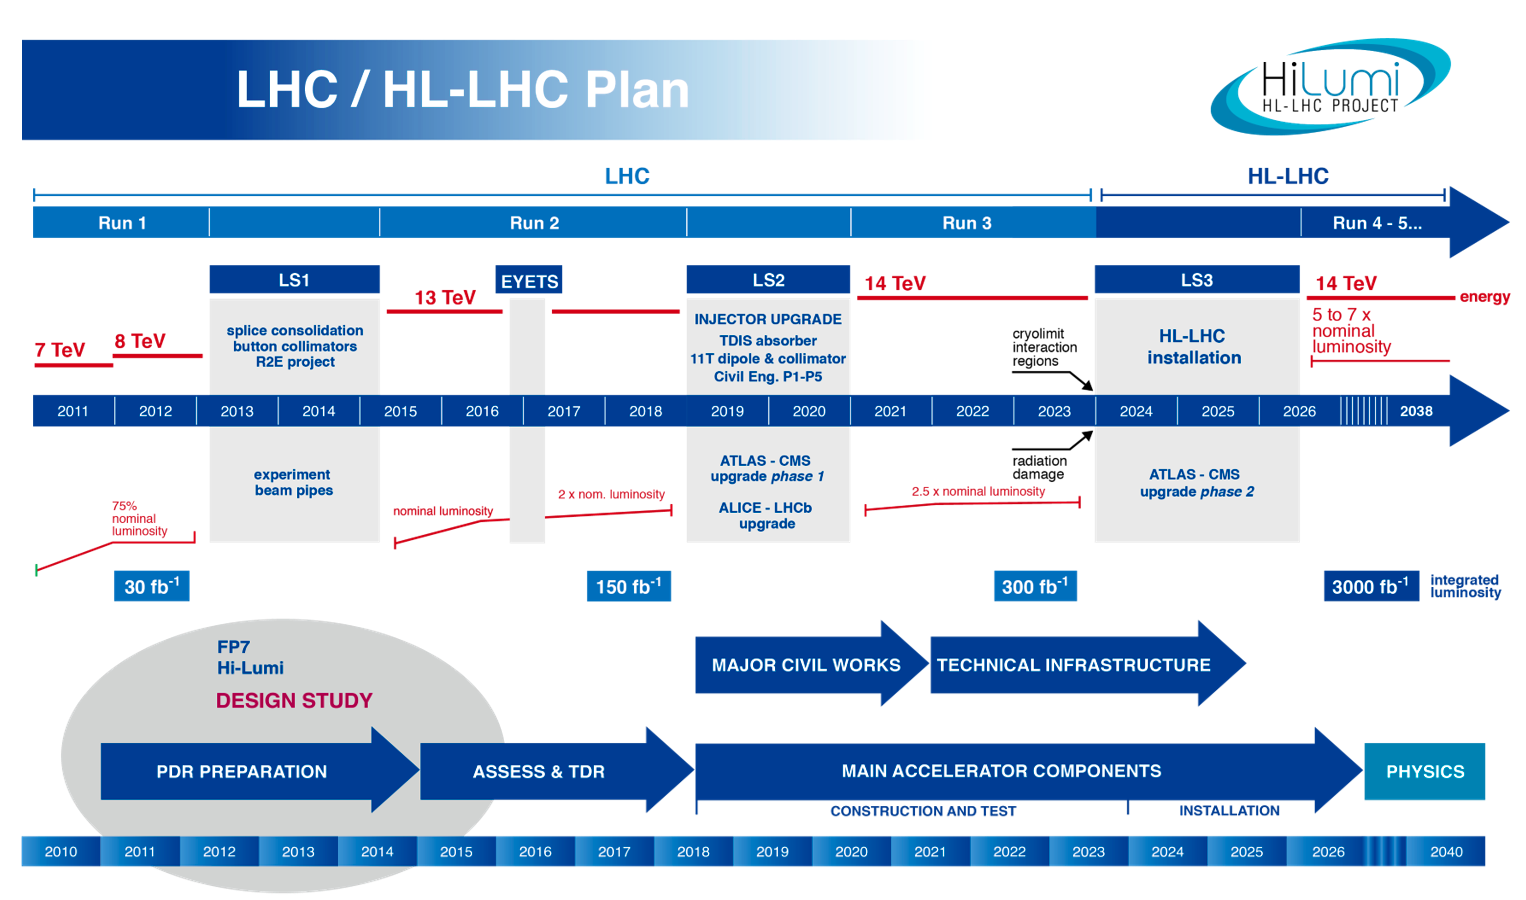
\includegraphics[width=0.9\textwidth]{Chapters/CH3/figures/phase2}
	\caption{Summary of the LHC timeline for operation and upgrade~\cite{phase2}.}
	\label{fig:phase2}
\end{figure}
\\At the end of 2018, the LHC was shut-down and for two years it will be upgraded to bring the center-of-mass energy to its design value of 14 TeV and collect 300 $\mathrm{fb^{-1}}$ of data, almost double the current available statistics of Run2.
After 4 years of duty cycle, the High-Luminosity period of LHC (HL-LHC) will start and aims to bring the integrated luminosity to 3000 $\mathrm{fb^{-1}}$, unlocking several studies, mostly related with rare phenomena, which are impossible to perform with the current datasets.\\
This chapter describes the Barrel Muon Trigger system (Section~\ref{barrel_muon_trig}), the BI upgrade for the HL-LHC (Section~\ref{BI_upg}), and the studies performed in the context of the RPC upgrade.
In particular, the goal of this work was the implementation of a new simulation to model the digitization of RPC hits in the BI region (Section~\ref{sec:hit_dig}) and, using this new model, trigger efficiency studies were performed in the BI and BM/BO regions (Section~\ref{sec:eff}).
In the end, summary and final considerations are also reported (Section~\ref{sec:concl_QT}).

\section{ATLAS Barrel Muon Trigger}
\label{barrel_muon_trig}
The muon detector chambers are arranged such that particles from the interaction point traverse three stations of chambers.\\
The system is subdivided azimuthally into 16 sectors numbered from 1 to 16.
The sector number increases in the direction of increasing $\mathrm{\phi}$ with the number 1 corresponding to coordinate $\mathrm{\phi=0}$. The odd sector (called “large sectors”)
are located between barrel coils, while, the even sectors (called “small sectors”) are covered by the coils.\\
The muon spectrometer consists of three large air-core superconducting toroidal magnets (two end-caps and one barrel) providing a field of approximately 0.5 T.\\
In the barrel, the chambers are arranged in three concentric cylinders around the beam axis called BI (Barrel Inner), BM (Barrel Middle), and BO (Barrel Outer). \\
The RPC planes are installed in the Middle
and Outer stations of the Muon Spectrometer and are mechanically associated with MDT precision chambers (except for some “special” chambers). \\
Schematic drawings of the present ATLAS MS~\cite{TDR}, are shown in Figures~\ref{fig:MS_rz} and~\ref{fig:MS_xy2}.
\begin{figure}[!h]
	\centering
	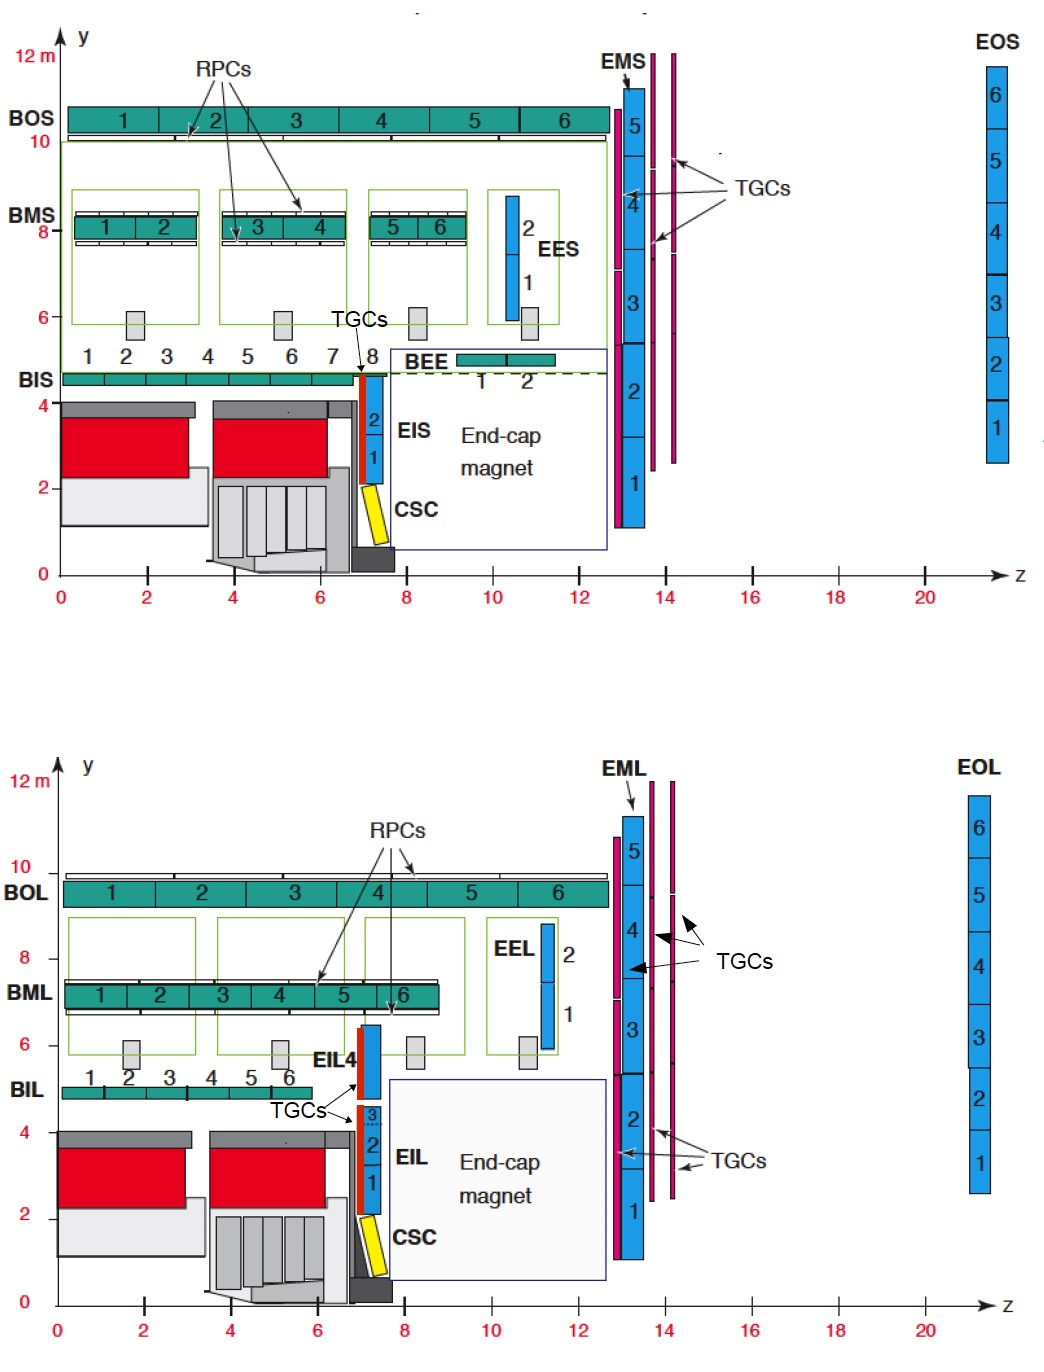
\includegraphics[width=0.9\textwidth]{Chapters/CH3/figures/MS_rz}
	\caption{Two R-Z views of the present (Run 1/2) ATLAS muon spectrometer layout. Top: One of the azimuthal sectors that contain the barrel toroid coils (small sector). Bottom: One of the sectors in-between the barrel toroid coils (large sector)~\cite{TDR}.}
	\label{fig:MS_rz}
\end{figure}
\begin{figure}[!h]
	\centering
	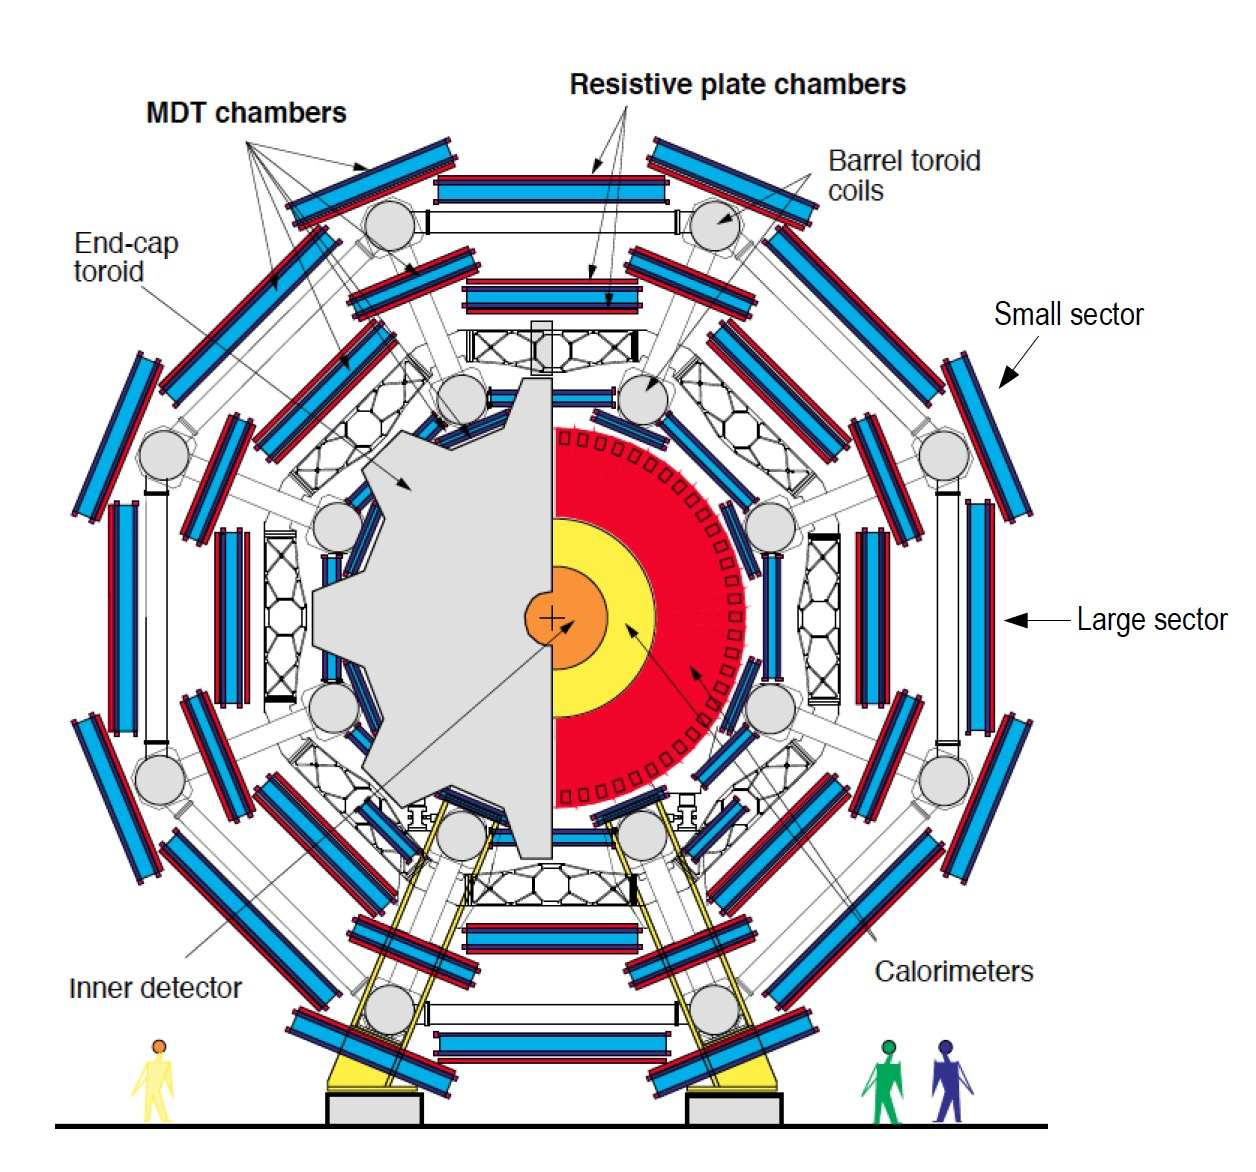
\includegraphics[width=0.9\textwidth]{Chapters/CH3/figures/MS_xy}
	\caption{View of the present (Run 1/2) ATLAS muon spectrometer barrel layout in the plane transverse to the beam axis (X-Y plane)~\cite{TDR}.}
	\label{fig:MS_xy2}
\end{figure}
The MS detector and electronics components have been designed for 10 years of operation
at a luminosity of $\mathrm{1\times 10^{34}cm^{-2} s^{-1}}$, corresponding to an integrated luminosity of 1000 \ifb. 
Conservative safety factors for radiation tolerance and rate capability were taken
into account in the original designs, and components have been tested up to and above
levels corresponding to the expected doses and rates predicted by simulations multiplied
by the safety factors. After the start of LHC operation, detector hit rates and radiation doses
could be measured directly, and the previous simulations have been found to agree with
the measurements to within a maximum deviation of about 50\%.
\\Based on this observation, the original safety factors were reduced [10], and as a consequence the original irradiation and high-rate tests have qualified the detectors for longer running and higher rates than originally anticipated.


\section {BI upgrade for Phase-II}
\label{BI_upg}
In the Phase-I upgrade, foreseen for LS2, the Small Wheels will be replaced by the New Small Wheels (NSW)~\cite{NSW} using small-strip TGC (sTGC) and Micro-Mesh Gaseous Structure
(MicroMeGaS or Micromegas, MM for short) chambers used for both triggering and precision tracking.\\
At the time of the Phase-II upgrade, there will thus be no CSC chambers
any more in the detector, nor will there be the Small Wheel MDT chambers, which are the ones closest to the beam line and exposed to the highest rates. Also in LS2, the BIS7 and
BIS8 MDT chambers will be replaced by integrated BIS78 stations of new RPC and small diameter MDT (sMDT) chambers to enhance the trigger coverage in this region~\cite{BIS78}.\\
Schematic drawings of the ATLAS MS with the new detectors that will be installed in the Phase-I and Phase-II upgrades are shown in Figure~\ref{fig:MS_rz_update}.\\
\begin{figure}
	\centering
	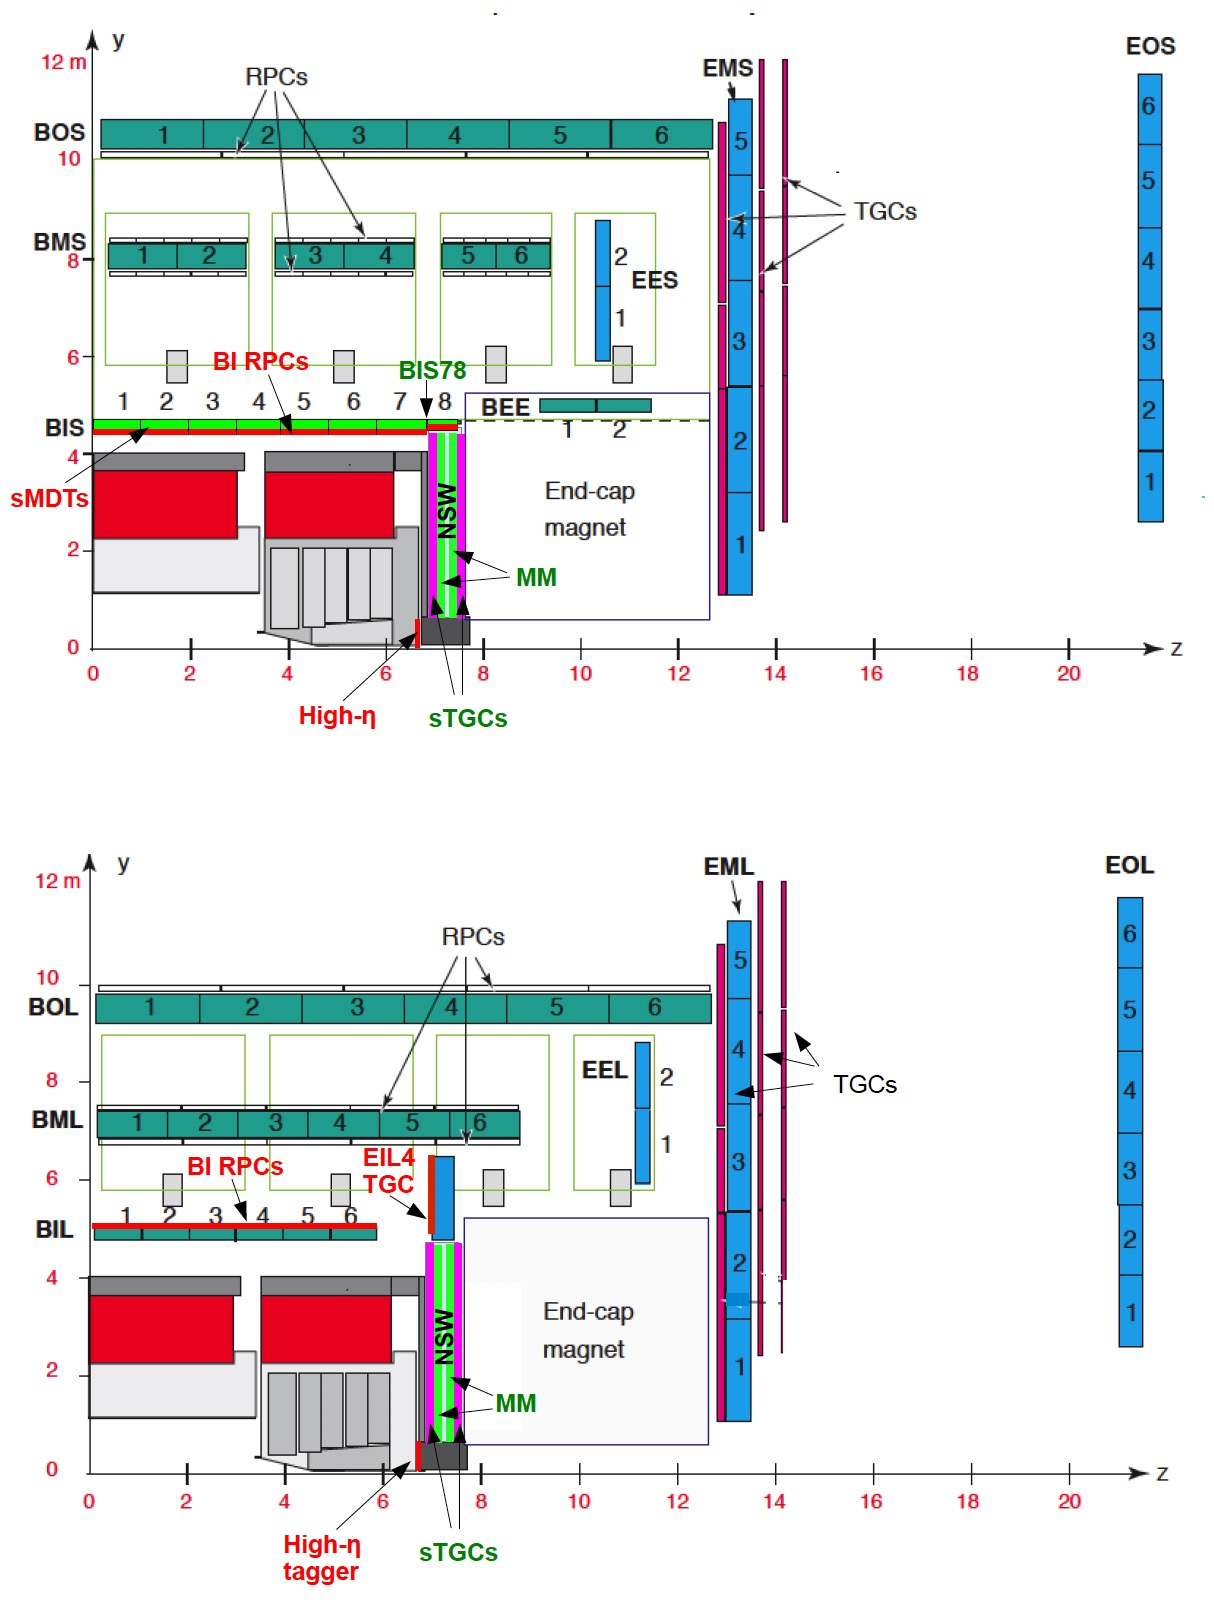
\includegraphics[width=0.9\textwidth]{Chapters/CH3/figures/MS_rz_update}
	\caption{Two R-Z views of the Phase-II ATLAS muon spectrometer layout showing a small sector (top) and a large sector (bottom). The drawings show the new detectors to be added in the Phase-II upgrade, including the addition of the high-$\mathrm{\eta}$ tagger (red text: BI RPC, sMDT, EIL4 TGC, high-$\mathrm{\eta}$ tagger), those to be installed during LS2 (green text: Micromegas and sTGC in the New Small Wheel and BIS78 RPC and sMDT), and those that will remain unchanged from the Run 1 layout (black text)~\cite{TDR}.}
	\label{fig:MS_rz_update}
\end{figure}

\noindent To maintain a high trigger efficiency, new RPC chambers with increased rate capability will be installed on the inner (BI) MDT chambers of the barrel. This addresses a fundamental issue
of the present (old) RPC chambers: to ensure their continued operation at the HL-LHC,
these chambers will have to be operated at reduced performance (i.e. efficiency), in order to
respect the original design limits on currents and integrated charge. This can be achieved
by reducing the gas gain through lowering the operating voltages. In the areas of high
backgrounds, the gas gain will have to be reduced to such low levels that hit inefficiencies
up to 35\% will be encountered. This would reduce the trigger efficiency in the barrel region
to an unacceptable level if no compensating measures were taken. In addition, due
to changes in regulations, the present gas mixture used in ATLAS RPCs may need to be
replaced by one with lower global-warming potential (GWP). Unless new gas mixtures are
found in time, this too will imply operation of old RPCs at a reduced efficiency. Despite
the lower single-hit efficiencies, a high trigger efficiency and purity can be maintained by
loosening the requirements on hit coincidences in the old chambers, if at the same time a
coincidence with the new BI RPC chambers is introduced. The installation of these chambers
will also close most of the acceptance holes of the present barrel muon trigger, which
amount to more than 20\% of the $\eta-\phi$ coverage for $!\eta!$ < 1.05 (see Section~\ref{sec:eff}).\\

\noindent Adding new RPC chambers in the barrel is challenging in terms of available space and
installation. In the small sectors, the BI RPC chambers can only be installed if the present
MDT chambers are replaced by new sMDT chambers with reduced overall thickness so that
the sMDT chambers and the new RPCs fit in the same envelope as the original MDT chambers.
In the large sectors there is sufficient space available to add the new RPC chambers
without replacing the MDTs, if on-detector services are re-arranged.\\
The retrofitting of selected RPC chambers in the BM and BO layer in the areas of high
rate at $|\eta|$ > 0.8, namely the BML7 and BOL6 chambers, is a small additional upgrade. The
MDT+RPC stations will be temporarily removed from the detector to replace the front-end
electronics and the readout panels, so that the chambers can be run at reduced HV without
efficiency loss. \\
In the Section~\ref{sec:BMBO_retrofit} it will be presented a study performed on the refurbish of
BM and BO chambers and the installation of BI chambers in the rail sectors 11 and 15.\\
The retrofitting can only be done outside the experimental cavern, on the
surface, since it requires the disassembly of the RPC chambers. The retrofitting of the BO
chambers does not fit into the LS3 schedule because it would interfere with the BI chamber
upgrade, and will likely be performed, at least partly, in winter shutdowns after LS3.\\


\noindent The main limitations of the RPC system for operation at the HL-LHC are related to the
chambers, owing to the more than a factor of seven higher luminosity than the chambers
were designed for. The RPC rate capability depends on the total charge delivered per count,
which, for the present RPCs, is 30 pC.\\
As a consequence, the single-gap efficiency will have to be reduced on average by 15\%, and by
35\% at large $\eta$. This efficiency loss will be compensated by installing a new layer of trigger chambers in the BI layer, increasing the overall barrel trigger redundancy.\\
To operate reliably at the HL-LHC, with high acceptance and efficiency and maintaining, the high trigger selectivity of the present system, several upgrades are required for the RPC system:
\begin{itemize}
	\item A new inner layer of BI RPC chambers will be added to the spectrometer. This will
recover most of the current geometrical acceptance holes. The redundancy of the
system will be greatly enhanced, so that full trigger efficiency can be maintained even
if the old RPCs have to be operated at reduced efficiency, either to limit the effects of
ageing or because the use of a different gas mixture is enforced. The BI RPCs will be
new-generation RPCs with 1 mm gas gaps and high-sensitivity front-end electronics.
	\item The trigger and readout electronics (Pad and splitter boxes) have to be replaced in order
to make the RPC system compliant with the Phase-II ATLAS trigger and readout
scheme. The entire electronics chain, except for the front-end boards, will be replaced.
The Pads will be replaced by the new data collector and transmitter (DCT) boards that
will send all data off the detector to the counting room USA15 where the trigger and
readout logic will be performed.
	\item In a worst-case scenario for the required reduction of efficiency of the old RPCs, a
reduction of the trigger efficiency may still occur even after the BI RPC installation,
in the region of $|\eta|$ > 0.8. This efficiency loss can be recovered by retrofitting a limited
number of BO chambers in that region. The retrofitting comprises replacing the
original front-end electronics by the new BI version, and replacing the readout strip
panels.
\end{itemize}
\newpage
\subsection{RPC upgrade}
The BI system is designed to increase the trigger acceptance and the trigger efficiency, by
loosening the requirements on the number of hits in the BM and BO chambers and, at the
same time, adding the requirement of a coincidence with the BI layer. Any coincidences of
hits in at least three chambers out of four (counting one BI, two BM, and one BO) will be
accepted. Two-chamber BI-BO coincidences will be used to cover the remaining acceptance
holes. Details of the Phase-II trigger algorithms and their performance are discussed in
Section~\ref{sec:trigScheme}. Figure~\ref{fig:tdr_eff} illustrates the recovery of acceptance and 
efficiency obtained with the Phase-II trigger including the BI RPCs in a worst-case scenario in 
which the single-hit efficiency of the old RPC is reduced by 15–35\% as a function of $|\eta|$, 
depending on the rate to which each chamber is exposed.
\begin{figure}[!h]
	\centering
	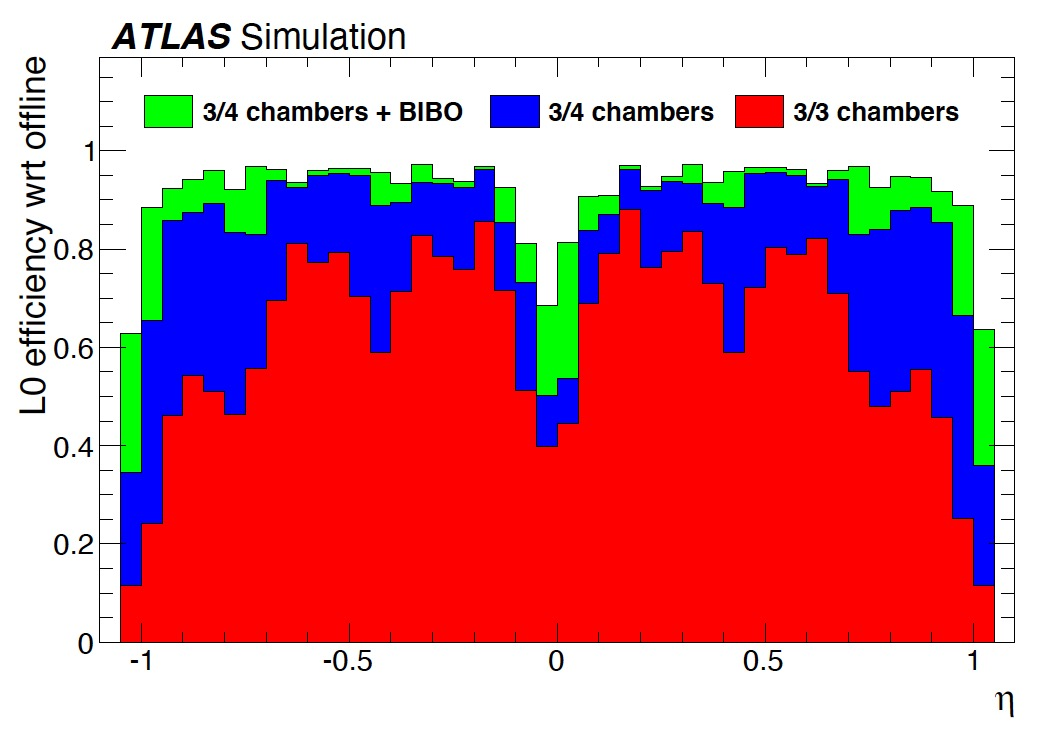
\includegraphics[width=0.9\textwidth]{Chapters/CH3/figures/tdr_eff}
	\caption{Efficiency times acceptance of the L0 barrel trigger for reconstructed muons with $p_{T} =
     25$ GeV as a function of $\eta$, assuming the worst-case scenario~\cite{TDR}.}
	\label{fig:tdr_eff}
\end{figure}
\\The new BI RPC chambers will have three sensitive gas gaps that are read out independently.
A majority logic requiring hits in at least two out of three planes provides high efficiency
while suppressing the rate of random coincidences due to uncorrelated hits from
photons and neutrons. This is necessary, for instance, to keep the rate of BI-BO coincidences
at an acceptable level.\\
A major re-design of the RPC technology started around the year 2010, mainly aiming at a
better rate capability and ageing behaviour. The new design is based on a reduced thickness
of the gas gaps (from 2 mm to 1 mm) and of the resistive electrodes (from 1.8 mm to
1 mm), and on the use of a new generation of low-noise high-sensitivity amplifiers. Using
these amplifiers, full efficiency can be achieved for a lower voltage across the gas gap, thus
transferring part of the amplification from the gas avalanche to the electronics. In this way,
the RPCs can be operated at a reduced charge per avalanche, reducing the detector current
and thus improving rate capability and ageing.\\
A detail view of the positions of the BI RPCs in ATLAS is shown in Figure~\ref{fig:xy_BIRPC}.
\begin{figure}[!h]
	\centering
	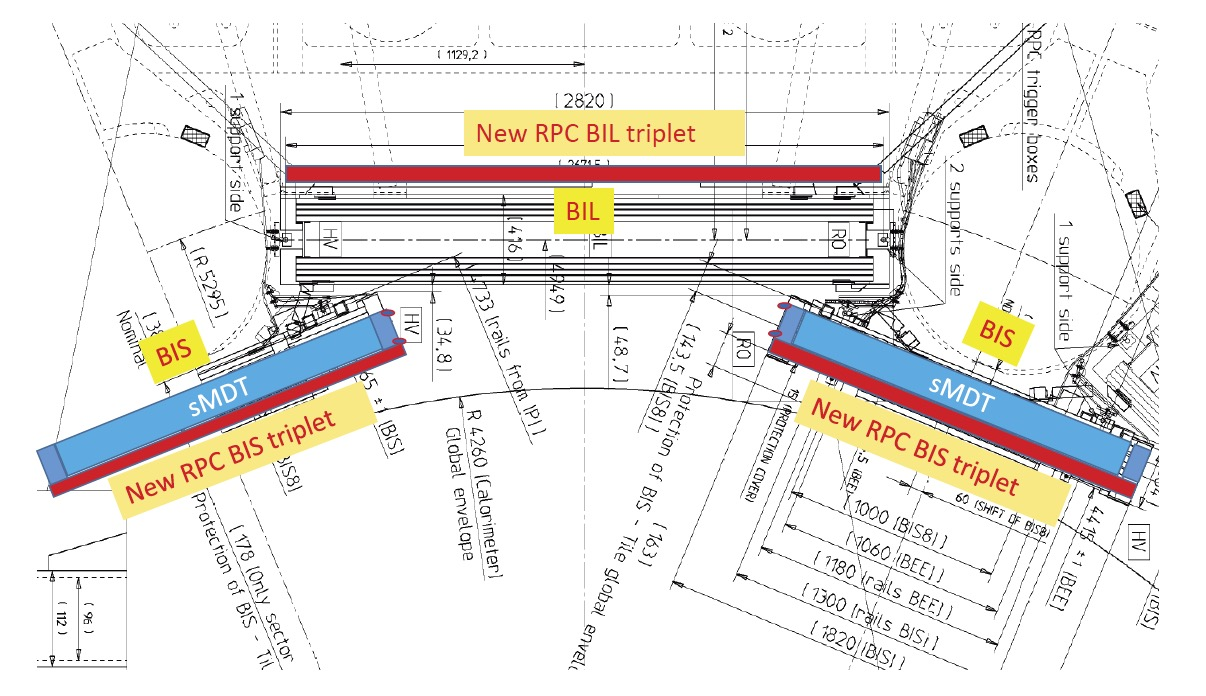
\includegraphics[width=0.9\textwidth]{Chapters/CH3/figures/xy_BIRPC}
	\caption{X-Y view of the inner barrel layer, indicating the positions of the BI RPCs (red) and BIS
sMDTs (blue) in the small and large sectors~\cite{TDR}.}
	\label{fig:xy_BIRPC}
\end{figure}
\\In the small sectors (BIS), due to the tight space limitations, the MDT chambers need to be 
replaced by new small-diameter MDT (sMDT) chambers with half the tube diameter (15 mm 
instead of 30 mm) in order to create space for the RPCs on the inside of the sMDT chambers. 
In  the large sectors (BIL), the new RPCs will be installed on the outside of the existing MDTs. The
layout of the new BI RPCs leaves the necessary holes and cut-outs for the existing MDT
alignment lines and for detector services. It comprises 272 triplet RPC chambers, for a total
area of about 470 $\mathrm{m^{2}}$. Acceptance studies based on a realistic description of the BI RPC geometry show a geometrical acceptance of the BI RPC chambers of 91\% for reconstructed muons with $|\eta|$ < 1.05, compared to 95\%  for the MDT chambers. This results in a barrel trigger acceptance of 96\%.\\
Each detector layer of the triplets is read out on both surfaces by orthogonal strip panels,
providing $\eta$ and $\phi$ measurements. The compact triplet structure and the use of highly
sensitive amplifiers require a complete isolation of individual layers from each other. The
choice of strip pitches, 24–26 mm depending on the chamber type, has been constrained
by the performance requirements, the strip impedance, and cost considerations. The total
number of readout channels is about 8700.

\subsection {Trigger scheme}
\label{sec:trigScheme}
All the hits from RPC detectors will be available to the barrel Sector Logic board that uses them to
generate barrel trigger candidates. The new BI RPCs increase the geometrical acceptance
of the present barrel muon trigger and its robustness against inefficiencies of the old BM
and BO RPCs caused by the reduced operating voltages necessary to ensure their longevity.\\
The RPC trigger will use nine measurement planes, provided by four layers of RPC chambers:
one BI triplet (RPC0), two BM doublets (RPC1 and RPC2), and one BO doublet (RPC3).
Figure~\ref{fig:trig_schemeXY} shows the positions of the BI, BM, and BO RPC chambers in a small 
barrel sector
together with the MDT chambers. The acceptance holes in the BM layer, caused by the
magnet coils and their supports, are also visible.
\begin{figure}[!h]
	\centering
	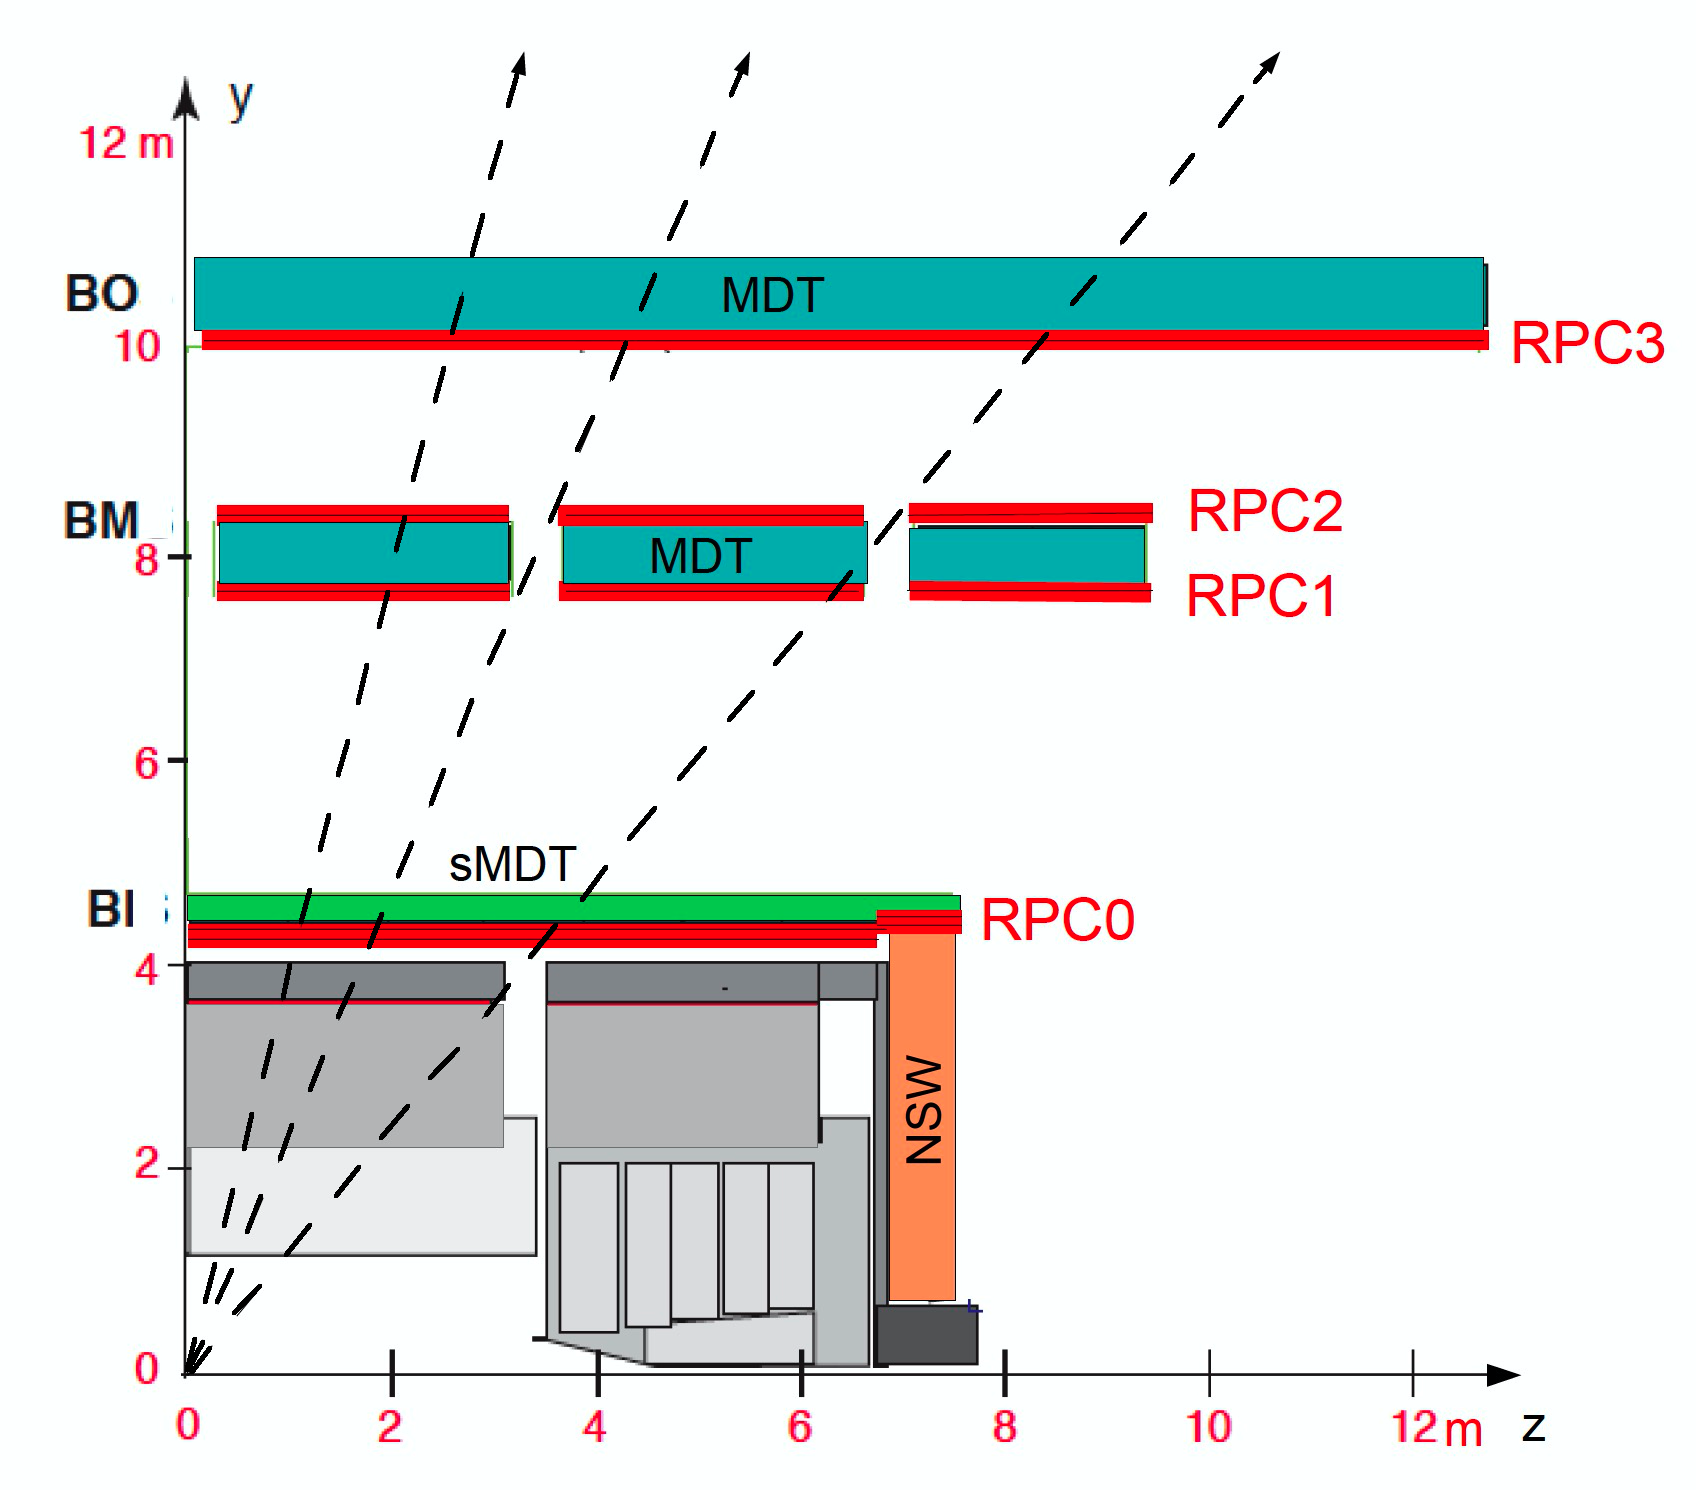
\includegraphics[width=0.75\textwidth]{Chapters/CH3/figures/trig_schemeXY_paint}
	\caption{Transverse section of a small sector in the barrel region, showing the four layers of RPC chambers (RPC0,1,2,3), as well as the MDT chambers in the barrel-inner (BI), barrel-middle (BM), and barrel-outer (BO) layers. The three dashed lines represent muon trajectories traversing four, two, and three RPC chambers~\cite{TDR}.}
	\label{fig:trig_schemeXY}
\end{figure}
\\To take advantage of the redundancy of detector planes, a trigger algorithm that does not
make use of a fixed pivot plane (as in present ATLAS muon trigger) has been developed.
This makes it possible to define different trigger coincidence logic schemes.\\ 
These schemes (summarised in Table~\ref{tab:trig_scheme} and illustrated in Figure~\ref{fig:trig_scheme}) are based on different requirements on the  four layers of RPC chambers:
\begin{itemize}
	\item 3/3 chambers. Hits in at least three out of four planes of the RPC1+RPC2 chambers
and in at least one out of two planes of RPC3. This is equivalent to the present high-pT
trigger.
	\item 3/4 chambers. The previous requirement in a logical OR with the requirement of
hits in at least two planes out of three in RPC0 and in at least three planes out of six
in RPC1+RPC2+RPC3. In this way, all combinations of three-chamber coincidences
(satisfying the above hit requirements) are accepted.
	\item 3/4 chambers + BI-BO. The previous requirement in a logical OR with the requirement
of at least two hits in RPC0 and at least one hit in RPC3. This enhances the
trigger coverage in the regions where no BM RPCs are installed due to the mechanical
support structure of the toroid coils. The BI-BO coincidence is expected to be
prone to accidental coincidences of uncorrelated background hits that are negligible
in three-chamber coincidences. In the baseline version of this trigger, BI-BO coincidences
are used in the whole barrel region, but can be limited to the BM acceptance
gaps, if the muon trigger rate in the barrel gets too high.
\end{itemize}
\begin{table}[h]
	\begin{center}
		\begin{tabular}{lp{0.75\textwidth}}
			\textbf{Trigger}  & \textbf{Requirement} \\
			\hline 
			3/3 chambers     & \scriptsize{\texttt{3[RPC1+RPC2] AND 1[RPC3]}} \\
			3/4 chambers     & \scriptsize{\texttt{(3[RPC1+RPC2] AND 1[RPC3]) OR (2[RPC0] AND 3[RPC1+RPC2+RPC3])}}\\
			3/4 ch.+BI\&BO    & \scriptsize{\texttt{(3[RPC1+RPC2] AND 1[RPC3]) OR (2[RPC0] AND 3[RPC1+RPC2+RPC3]) \hspace{2cm} OR (2[RPC0] AND 1[RPC3])}}\\
			\hline 
		\end{tabular} 
		\caption{The hit requirements used in different RPC triggers. The left column shows the short name used in the text. The right column gives the coincidence scheme used for the selection logic. The notation \texttt{N[RPCi+RPCj+...]} indicates a majority requirement of hits in at least N planes out of all the possible planes available in RPC chambers RPCi, RPCj, . . . with \textit{i, j,} . . . \textit{$\in$} $\{0, 1, 2, 3\}$.} 
		\label{tab:trig_scheme}
	\end{center} 
\end{table} 
\begin{figure}[!h]
	\centering
	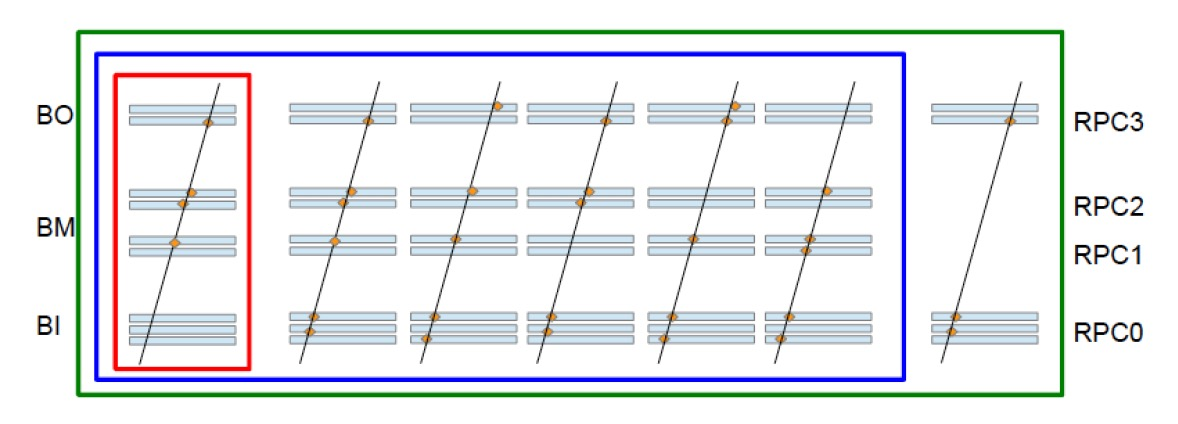
\includegraphics[width=0.8\textwidth]{Chapters/CH3/figures/trig_scheme}
	\caption{Graphic view of the coincidence scheme used for the selection logic. High-Pt (3/3 chambers) in red, 3/4 chambers in blue, 3/4 ch.+BI\&BO in green.}
	\label{fig:trig_scheme}
\end{figure}

\section{Hit digitization in the BI region}
\label{sec:hit_dig}
Since at the present time the new chambers in the BI region are not yet installed,
the simulation performed for this work takes into account the presence 
of hits in the BI RPC chambers exploiting the true hits, recorded 
by the MDT chambers in the BI region, and treating them as hits of the future RPC chambers.\\
In this work, it has been used the the common framework \texttt{muTrigNt\_write}~\cite{muTrigNt} that includes a realistic digitization.
This code reproduces the dimensions of the new BI RPC chambers and, 
given as input the true MDT hits, it checks if the hits are in the geometric 
acceptance.
The code also allows to generate strips, of an arbitrary pitch, in the two orthogonal directions ($\eta$ and $\phi$) and thus to digitize the true MDT hits, recording them as hits with the coordinates reported in the center of the strip.
In this way, it is possible to completely simulate the RPC chamber. \\
%This \texttt{muTrigNt\_write} is also able to simulate the trigger efficiencies, as described in Sec~\ref{sec:eff}. 
The studies presented in this chapter were performed using the official MC sample\\  {\scriptsize\texttt{mc15\_14TeV.422063.ParticleGun\_single\_mu\_Pt50.recon.ESD.e5392\_s2988\_s3000\_r8974}}~\cite{Muontwiki}, containing 50K events, produced with the ITk (Inner Tracker) simulation and with the layout of Run-I muons, that differs compared to the layout of Run-II muons because the feet and the elevator chambers are missing.
This MC sample considers muons reconstructed in $|\eta| < 1.05$ by the offline reconstruction, using a single-muon MC sample with fixed \mbox{$p_{T}=50$ \GeV}. \\
Given the framework described above, the goal of this work was to implement a simulation with a more realistic digitization that would produce:
\begin{itemize}
	\item cluster size, strip number and the associated coordinates of the strips (Section~\ref{sec:CSM});
	\item timing (Section~\ref{sec:timing});
	%\item the option of BI RPCs with two-sides $\eta-\eta$ readout  (Section~\ref{sec:etaeta});
%	\item BI and BMBO Efficiencies (Section~\ref{sec:eff});
\end{itemize}

\subsection{The cluster size model}
\label{sec:CSM}
A single discharge in the gas volume can induce a signal in more than
one RPC strip (i.e. it causes a so-called $cluster$), which is due to the charge sharing.
The number of the RPC strips fired in temporal coincidence is called $cluster$ $size$. 
The cluster size is a relevant parameter for the RPC detector and it must be strictly monitored to 
ensure a full trigger efficiency,
The cluster size is simulated using a Gaussian charge distribution, with fixed width and centered on the true MDT hit that is induced on the strips~\cite{MuonWeek22Oct}. 
This function is defined as:
\begin{equation}
G(z)=A(z)\cdot \frac{2}{\pi} \int{e^{-\frac{\mu-z}{\sigma\sqrt{2}}}}
\end{equation}
where the amplitude $A(z)$ is a random distribution having a decreasing exponential distribution  $f(A)=e^{-\frac{z}{\tau}}$, with the parameter $\tau$ = 0.8, fixed width $\sigma$ = 16 mm and $\mu$ is the $z$~-~coordinate of the hit.
When the charge integrated over a strip exceeds a certain threshold (0.2 in this simulation), the strip is switched on.\\
This is not a strictly physical model but a decreasing exponential is useful to produce the expected tail, in the absence of a more realistic model for amplitudes
based on experimental studies. A picture of the model used in this simulation is illustrated in Figure~\ref{fig:csm_pic}.
\begin{figure}[!h]
	\centering
	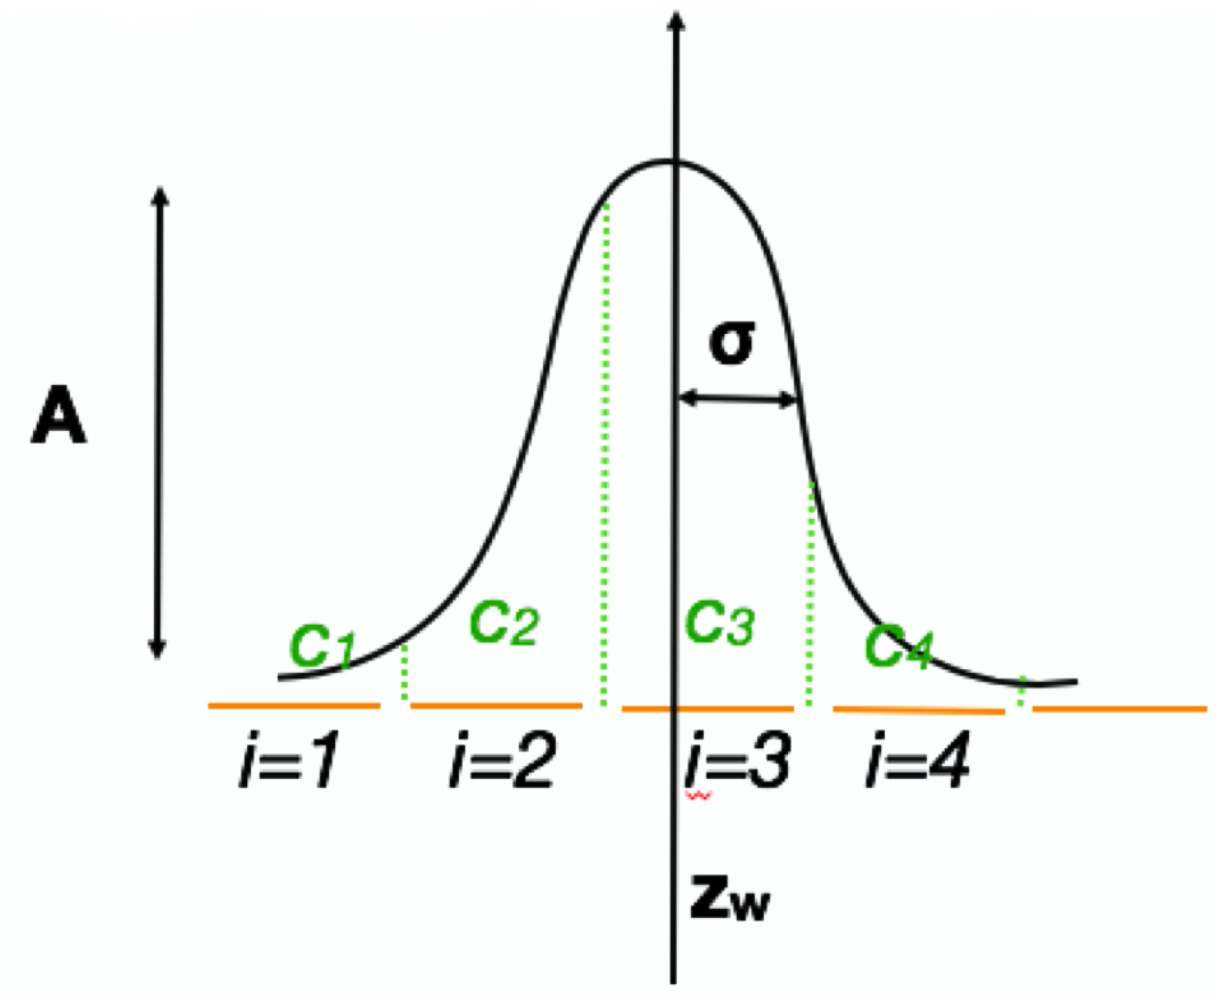
\includegraphics[width=0.53\textwidth]{Chapters/CH3/figures/csm_pic}
	\caption{Cluster size model used in the simulation. $C_i$ is the charge integrated over a strip $i$. 
		Some other parameters are the strip pitch $z_w$ ( 22 mm), random amplitude$A$ and width $\sigma$. When the charge integrated over a strip exceeds a certain threshold, the strip is switched on~\cite{MuonWeek22Oct}.}
	\label{fig:csm_pic}
\end{figure}
Cluster size is given by the number of strips fired at the same time. \\
It depends on the absolute value of charge integrated over a strip, but it also depends on the position of the true hit.
Originally, the RPC hit is fixed to be at the center of the strip and the true MDT hit belongs to one strip only but in this simulation, it would be possible to have many strips fired at the same time using the relation: $\mathrm{GlobPos_{i} = GlobPos_{i,true}\pm strip\_center_{i}}$. 
The resulting cluster size distribution is in line with the expectations in~\cite{TDR} and shown in Figure~\ref{fig:CS}.
\begin{figure}[!h]
	\centering
	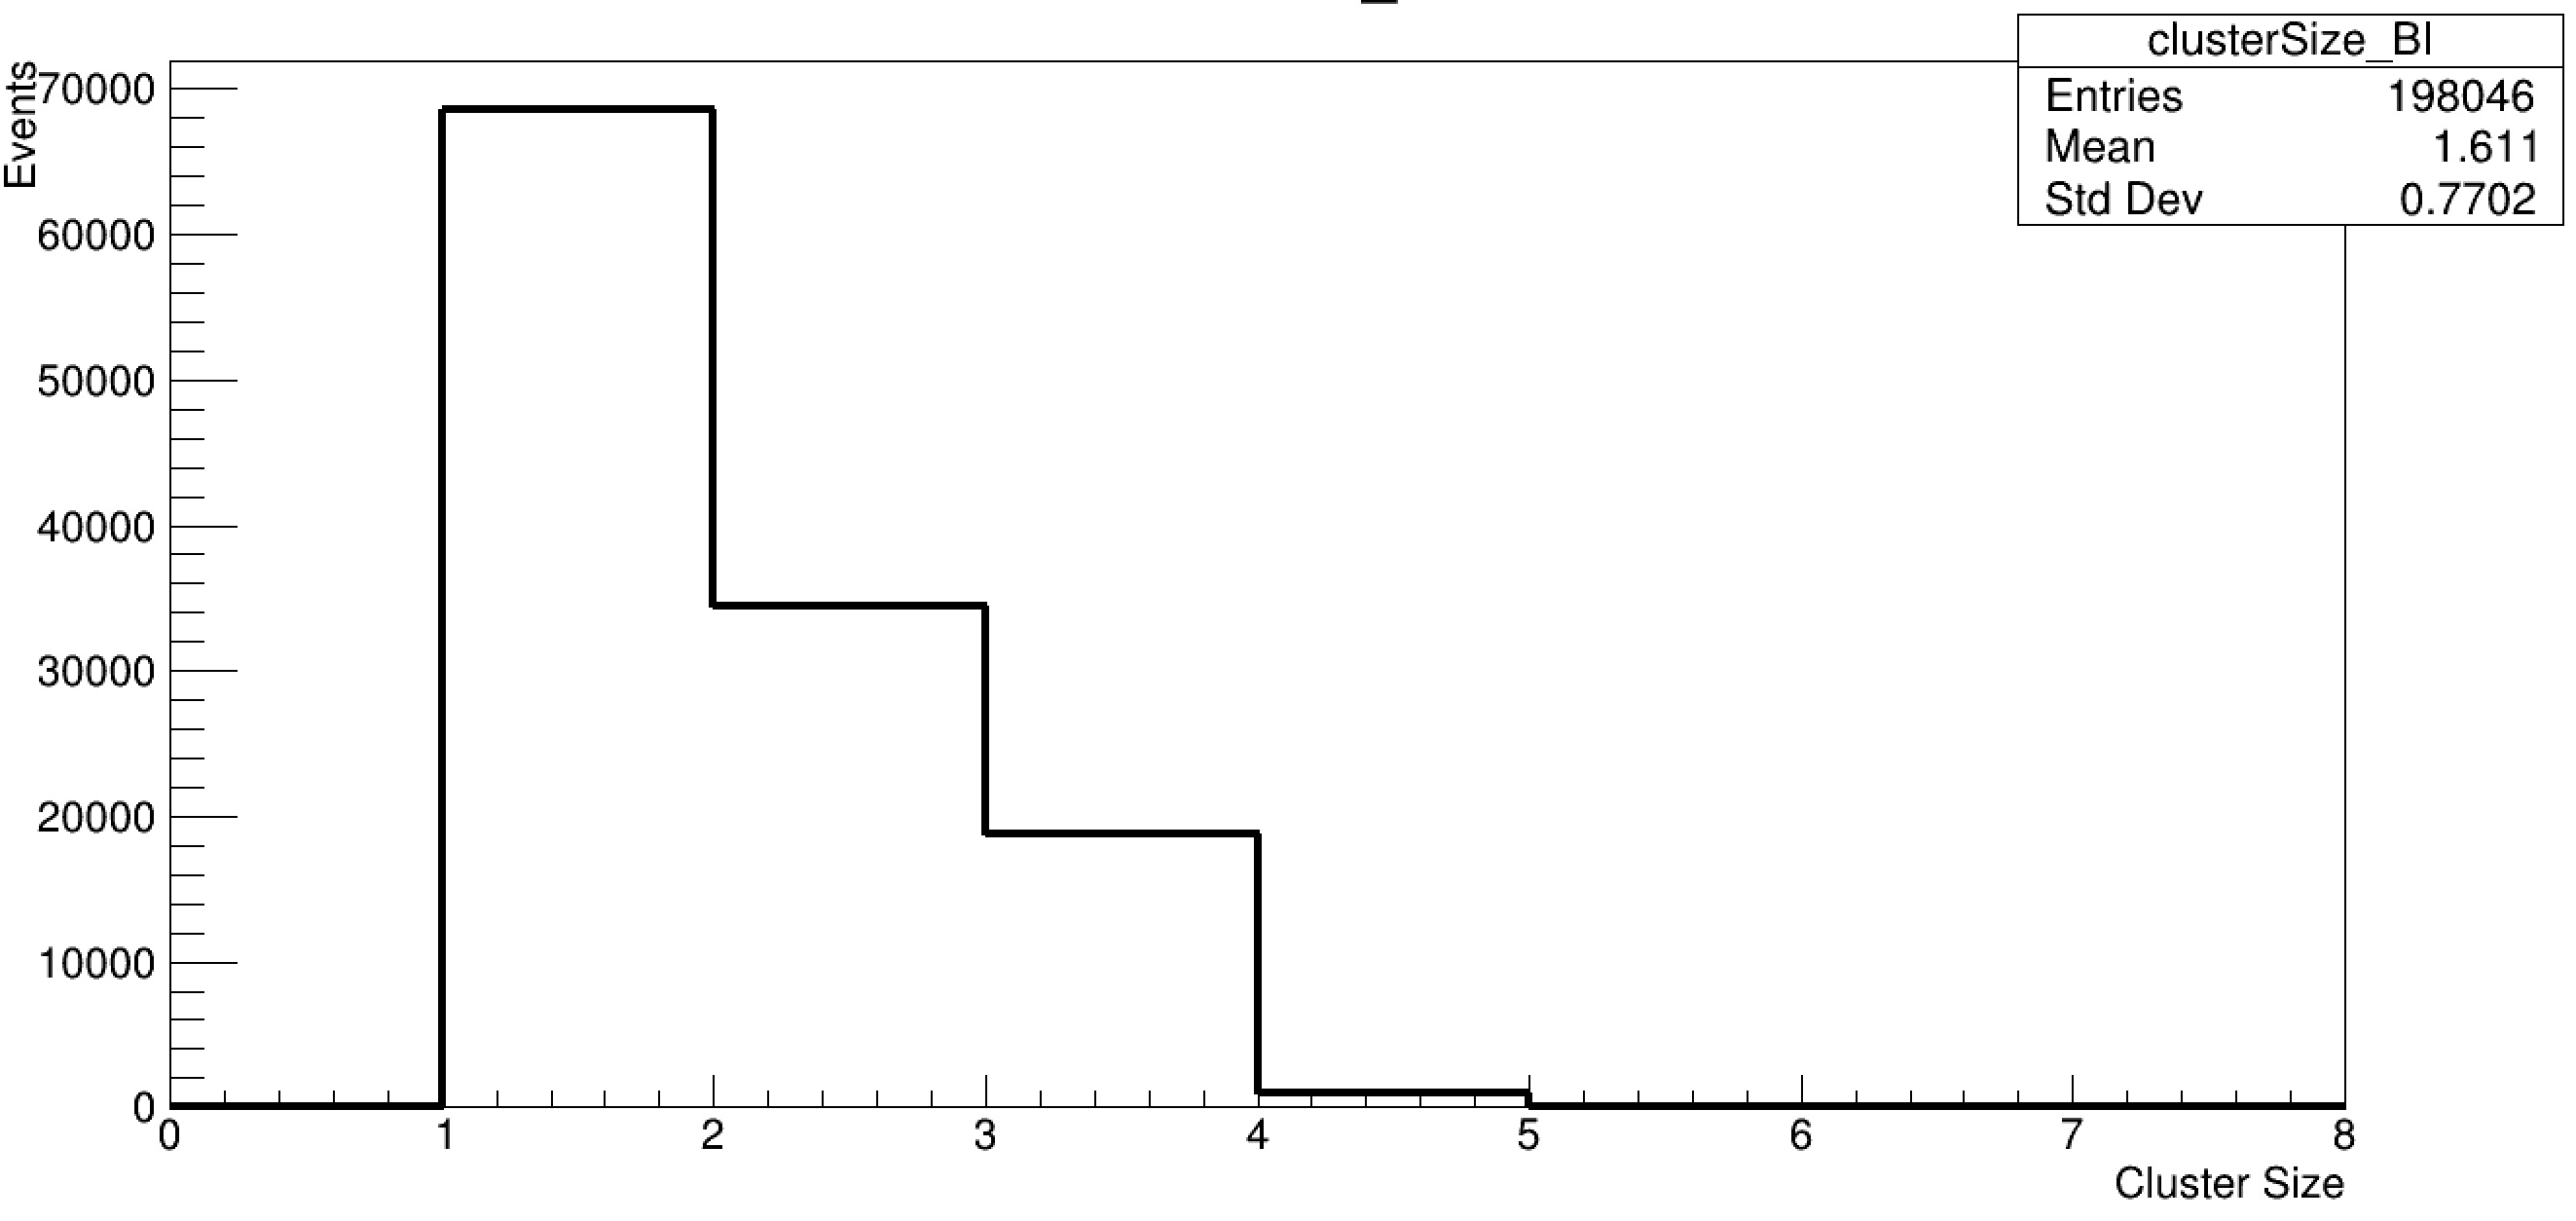
\includegraphics[width=0.7\textwidth]{Chapters/CH3/figures/CS}
	\caption{Cluster size distribution obtained with the model and parameters illustrated in this section. The average value is 1.6.}
	\label{fig:CS}
\end{figure}
\newpage\phantom{}
\noindent Considering the hit distribution in Figure~\ref{fig:strips_eta} for the $\eta$ layer and Figure~\ref{fig:strips_phi} for the $\phi$ layer, it is possible to see that:
\begin{itemize}
\item CS=0 is never possible by definition, one hit corresponds to at least one fired strip;
\item CS=1 the hit distribution is uniform, because the integrated charge is less than the fixed threshold;
\item CS=2 mostly when the truth hit is far from the strip center and at the strip~edge;
\item CS=3 mostly when the truth hit is far from the strip~edge and at the strip~center;
\item CS=4 mostly when the truth hit is far from the strip center and at the strip~edge.
\end{itemize}
\begin{figure}[!h]
	\centering	
	\subfigure[] {\label{fig:strips_eta}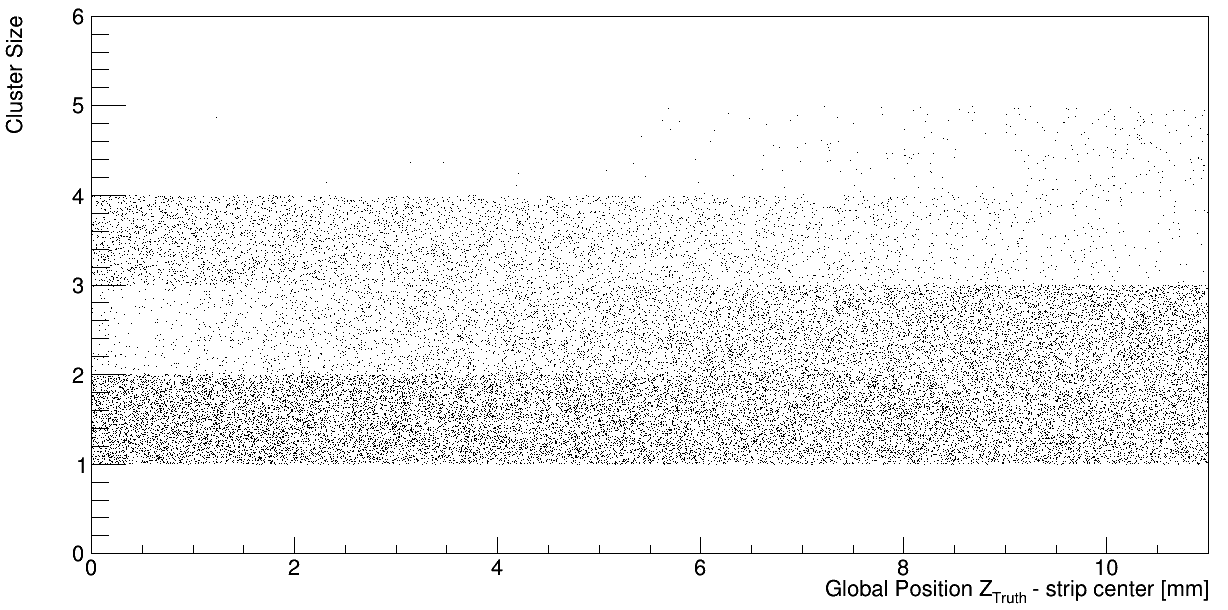
\includegraphics[width=0.83 \textwidth]{Chapters/CH3/figures/clusterSize_BI_stripCenterEta}} 
	\subfigure[] {\label{fig:strips_phi}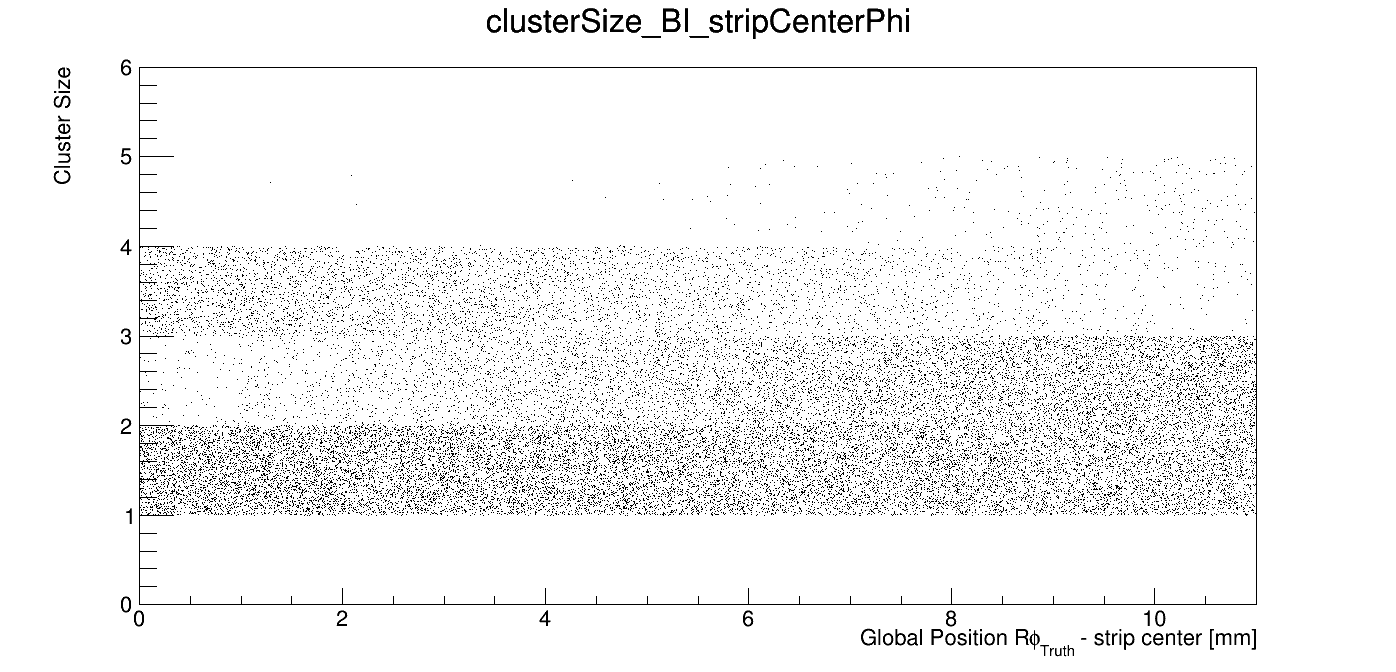
\includegraphics[width=0.83 \textwidth]{Chapters/CH3/figures/clusterSize_BI_stripCenterPhi}} 
	\caption{RPC hit distribution $\mathrm{GlobPos_{i}}$ for \subref{fig:strips_eta} strips along $\eta$ and \subref{fig:strips_phi} strips along $R\phi$.}
	\label{fig:strips}
\end{figure}	
Strips in $\eta$ and $\phi$ layers are orthogonal to each other and it is possible to see how 
they are arranged as a function of the Global Position in the BI region of the ATLAS detector.\\
In particular, in Figure ~\ref{fig:Nstrips_eta} strips oriented along $\eta$ are ordered in such a 
way that the strip number one is the inner strip, while Figure ~\ref{fig:Nstrips_phi} shows that 
strips oriented along $\phi$ are always oriented with increasing $\phi$. 
\begin{figure}[!h]
	\centering	
	\subfigure[] {\label{fig:Nstrips_eta}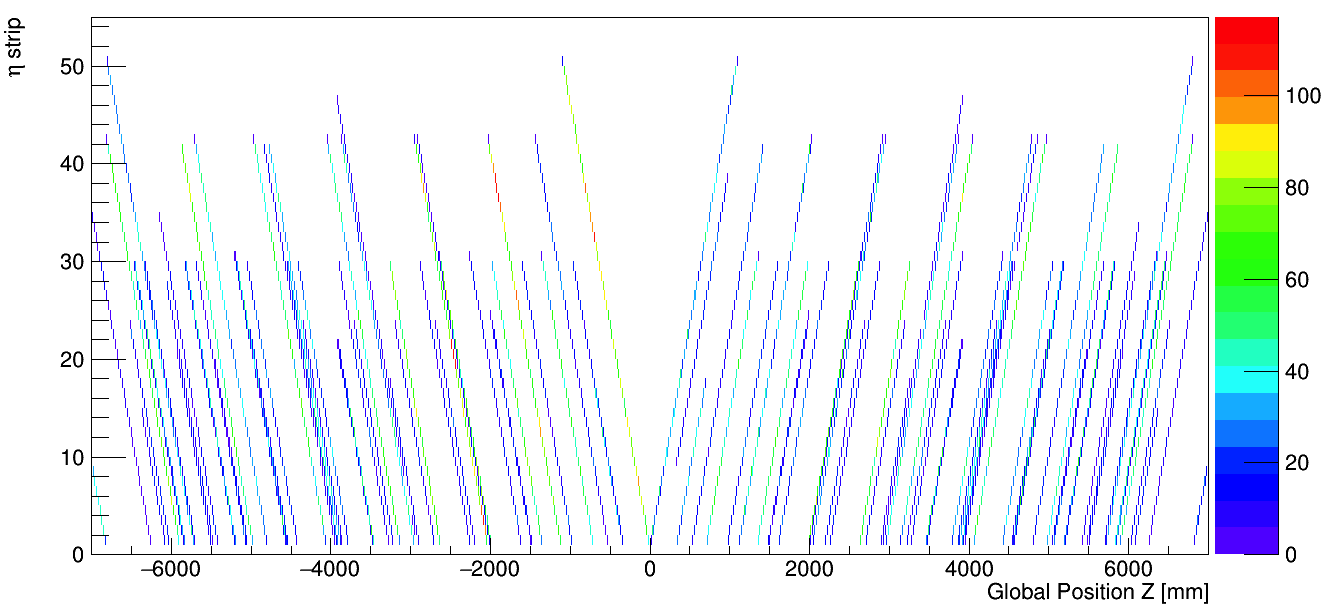
\includegraphics[width=1 \textwidth]{Chapters/CH3/figures/h_globalPos_StripEta}} 
	\subfigure[] {\label{fig:Nstrips_phi}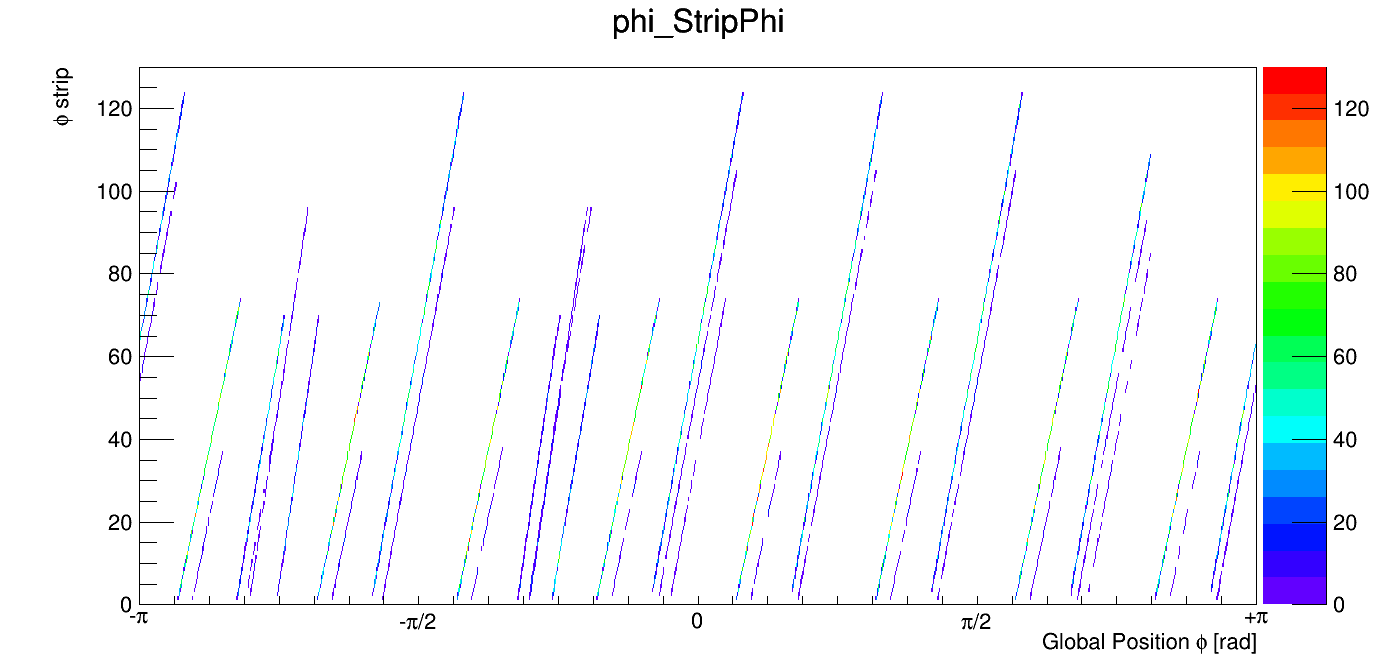
\includegraphics[width=1 \textwidth]{Chapters/CH3/figures/h_phi_StripPhi}} 
	\caption{Arrangement of strips in the \subref{fig:Nstrips_eta} $\eta$ layer and \subref{fig:Nstrips_phi} $\phi$ layer as a function of the Global Position in the BI region of the ATLAS detector.}
	\label{fig:Nstrips}
\end{figure}	
\newpage
\noindent \Cref{fig:param_BIL,fig:param_BIR} summarises the main chamber parameters of the expected layout 
for the Phase-II upgrade. Strip and front-end board 
entries are based on the assumptions of a 20 mm pitch and eight channels per board.\\
Figure~\ref{fig:strips_BI} shows the number of $\eta$ and $\phi$ strips switched on in the 
simulation. It is possible to verify that the simulation developed for this work follows the requirements of the Phase-II upgrade for BI RPCs to be realistic and reliable as much as possible.
\begin{table}[!h]
	\centering	
	\subfigure[] {\label{fig:param_BIL}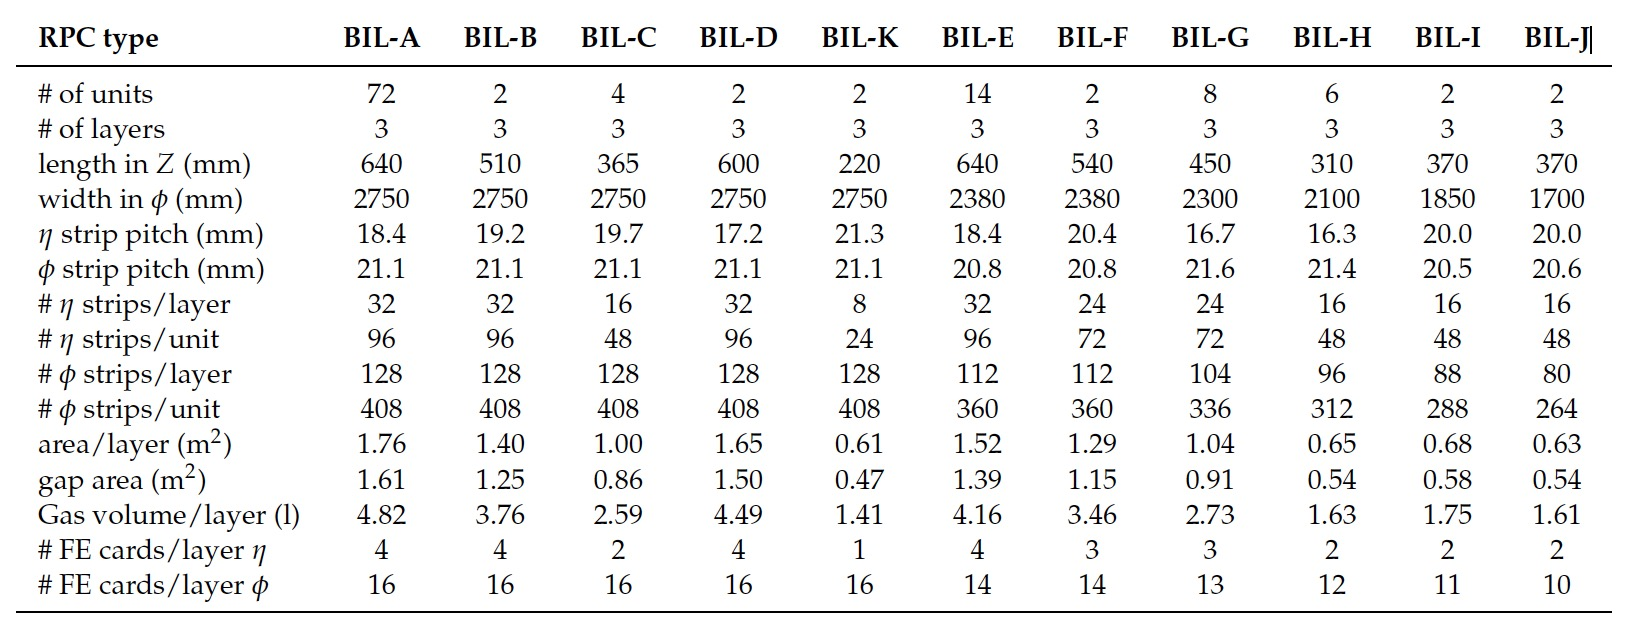
\includegraphics[width=1 \textwidth]{Chapters/CH3/figures/param_BIL}} 
	\subfigure[] {\label{fig:param_BIR}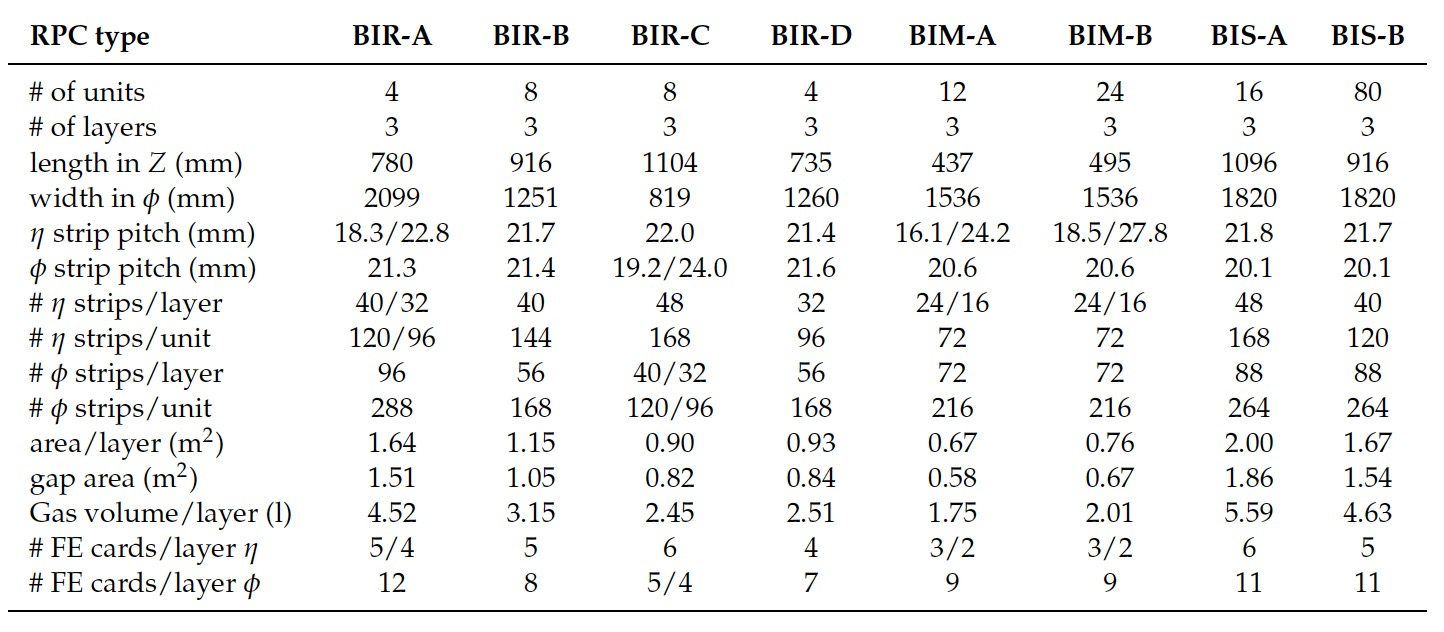
\includegraphics[width=1 \textwidth]{Chapters/CH3/figures/param_BIR}} 
	\caption{Main parameters of \subref{fig:param_BIL} the BIL RPC chambers and \subref{fig:param_BIR} the BIR/BIM/BIS RPC chambers~\cite{TDR}.}
	\label{fig:param}
\end{table}	
\begin{figure}[!h]
	\centering	
	\subfigure[] {\label{fig:CS_eta}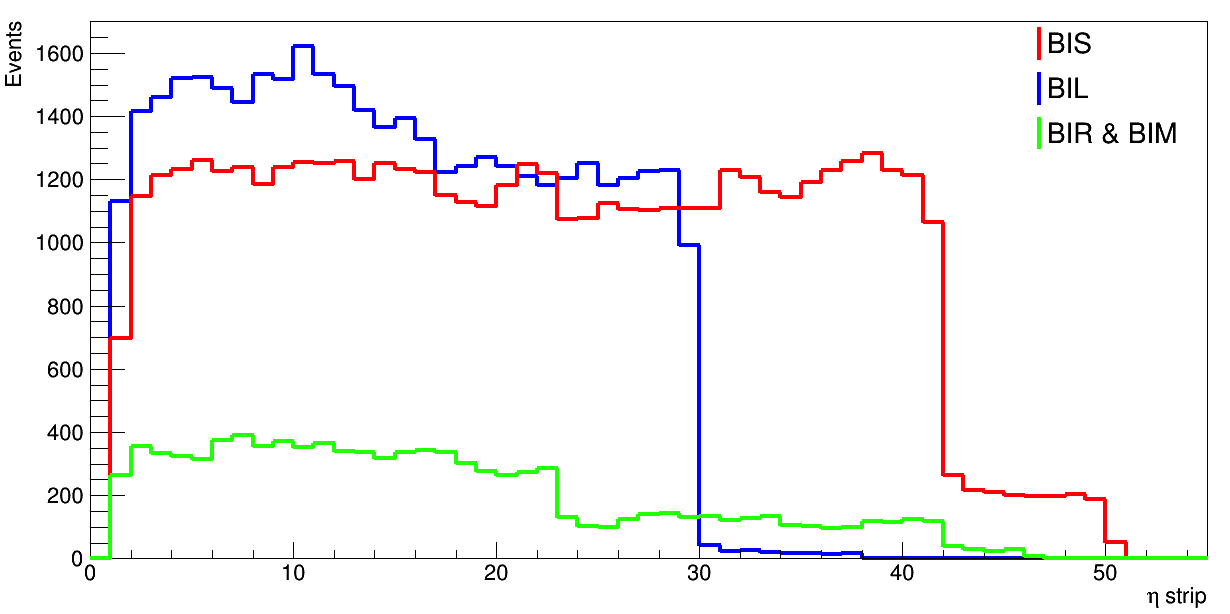
\includegraphics[width=0.95 \textwidth]{Chapters/CH3/figures/stripEta_BI}} 
	\subfigure[] {\label{fig:CS_phi}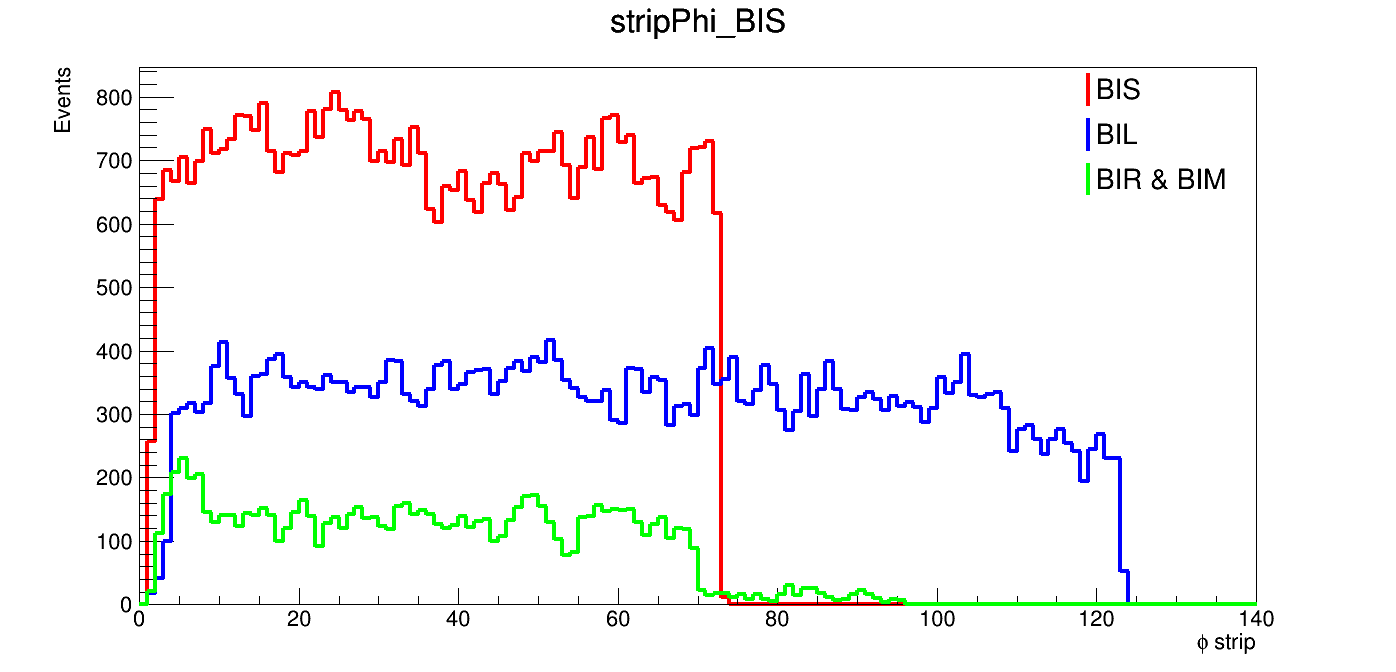
\includegraphics[width=0.95 \textwidth]{Chapters/CH3/figures/stripPhi_BI}} 
	\caption{Number of $\eta$ and $\phi$ strips switched on for different chambers:  BIS in red, BIL in blue, BIR \& BIM in green.}
	\label{fig:strips_BI}
\end{figure}	
\FloatBarrier

\subsection{Timing}
\label{sec:timing}
Another important variable is the time taken for the particle to pass through the detector. It is 
important because it is one of the discriminating variables in the algorithm's selection of hits. 
Only hits recorded in the bunch crossing event are considered and not all the hits previously recorded. 
Therefore, all hits outside 25~ns coincidence window around the bunch crossing of interest are 
excluded.\\
In order to simulate the new RPCs one has to take into account several effects and apply an 
appropriate correction and extract a digital readout.
\vspace{\baselineskip}\\
The final formula used to extract the digitized time in which the hit is recorded by the detector is:
\begin{equation}
t_{hit}= int\footnotemark\bigg\{\frac{t_{true}+t_{Gauss}+t_{FE}-t_{cal}}{\Delta t}\bigg\}\Delta t
\label{eq:timing}
\end{equation}
\begin{itemize}
	\item $t_{true}$ is the true hit recorded by the MDT;
	\item $\Delta t$ is the sampling rate (0.3 ns). The final $t_{hit}$ must be a multiple of the sampling rate to have a digitization;
	\item $t_{Gauss}$ is a Gaussian term that reproduces the fluctuations in the RPC signal 
	(smearing 0.4 ns);
	\item $t_{FE}$ is the propagation of the signal along the strip to the FE electronics 
	assuming  that the signal speed on the layer is 200 mm/ns;
	\item $t_{cal}$ is the calibration offset. The true hit timing is recorded referring to the time 
	of the collision on the MDT tubes. To report the timing centered around 0, it was necessary to 
	subtract the time of flight of the particle assuming time to be calibrated with 
	prompt muons crossing the center of the strip at t = 0.
\vspace{\baselineskip}\\	
Figure~\ref{fig:time_BI} shows the digitized time associated to the RPC hit calculated using the 
Equation~\ref{eq:timing}. The tail of the distribution is given by low $p_T$ muons  that produce 
secondary hits.
\end{itemize} 

\begin{figure}[!h]
	\centering
	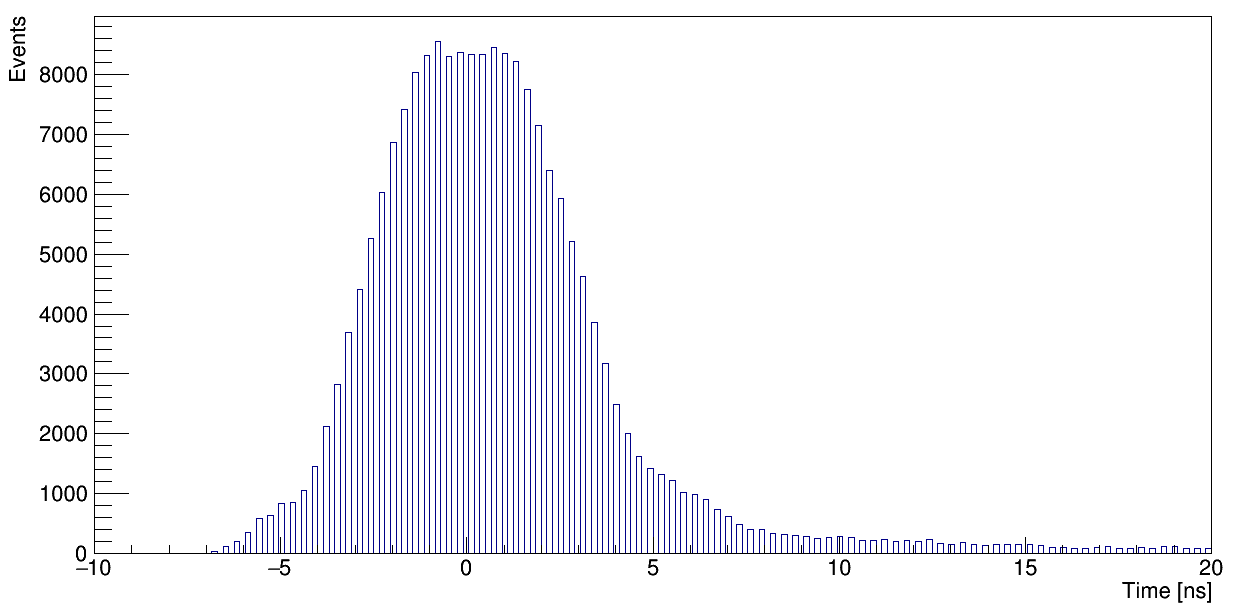
\includegraphics[width=0.9\textwidth]{Chapters/CH3/figures/time_BI}
	\caption{Digitized time associated to the RPC hit. The tail of the distribution is given by low 
		$p_T$ muons that produce secondary hits}
	\label{fig:time_BI}
\end{figure}

\footnotetext{The $int$ function takes the integer part of a real number.}

\section{L0 barrel trigger efficiency}
\label{sec:eff}
The performance of the barrel muon trigger was studied using single-muon MC samples with fixed \pT = 50 \GeV, for a fixed transverse momentum threshold: $p_{T} > 10$ GeV~\cite{Marcoccia:2693982} and with the hit digitization described in the previous sections.\\
To study the robustness of the trigger against possible efficiency reductions of the old RPCs in the BM and BO layers, the simulation was performed in the so-called "worst-case scenario" that introduces inefficiencies depending on the station type and sector and summarised as Table~\ref{tab:WCS}. It includes inefficiencies due to a reduction of the high voltage of the BM and BO RPCs such that the expected RPC current is always below the safe operation limit.
\begin{table}[htbp]
	\begin{center}
		\begin{tabular}{c|cccccccc}
			\multirow{2}{*}{\textbf{Station Name}} & \multicolumn{8}{c}{\textbf{StationEta}}\\
			\cline{2-9}
			& \textbf{1} & \textbf{2} & \textbf{3} & \textbf{4} & \textbf{5} & \textbf{6} & \textbf{7} & \textbf{8}\\
			\hline 
			BOL                 				   & 0.90  	    & 0.90		 & 0.82 	  & 0.82 	   & 0.76 		& 0.74 		 & -	      & -    \\
			BOS/BOG/BOF 						   & 0.89 		& 0.90 		 & 0.90 	  & 0.90	   & 0.89 		& 0.66 		 & 0.60       & 0.60 \\
			BML                					   & 0.88		& 0.88 		 & 0.88 	  & 0.83 	   & 0.56 		& 0.56		 & 0.60       & -    \\
			BMS              					   & 0.90  	    & 0.90		 & 0.90 	  & 0.87 	   & 0.81 	    & 0.81    	 & -          & -    \\
			\hline 
		\end{tabular} 
		\caption{Efficiency for each station and sector of the barrel muon trigger in the "worst-case scenario". This scenario includes inefficiencies due to a reduction of the HV of the BM and BO RPC~\cite{Marcoccia:2693982}.} 
		\label{tab:WCS}
	\end{center} 
\end{table} 
\noindent The trigger efficiency times acceptance for each trigger logic scheme is listed in Table~\ref{tab:eff_x_acc_wcs} and it is defined as the fraction of reconstructed muons that are accepted by the trigger, using the simulation that includes the RPC detector efficiency.
The trigger efficiency times acceptance is also presented in Figure~\ref{fig:h_eff}. 
Adding the new BI RPC layer greatly reduces the dependence of the trigger efficiency on the hit efficiency of the old RPCs.
\begin{table}[h]
		\small
\begin{tabular}{l|c|c|c}
	\hline
	\multirow{2}{*}{\textbf{BM and BO efficiency (\%)}} & \multicolumn{3}{c}{\textbf{Trigger efficiency x acceptance (\%)}}\\
	\cline{2-4}   
	& \textbf{3/3 chambers} & \textbf{3/4 chambers} & \textbf{3/4 chambers + BIBO}\\
	\hline 
	WCS 												& 58.78 				& 83.27 		& 91.89\\
	\hline 
\end{tabular} 
\caption{Efficiency times acceptance for the L0 barrel trigger for each trigger logic scheme, assuming the worst-case scenario with the hit digitization  .} 
\label{tab:eff_x_acc_wcs}
\end{table} 
\begin{figure}[!h]
	\centering
	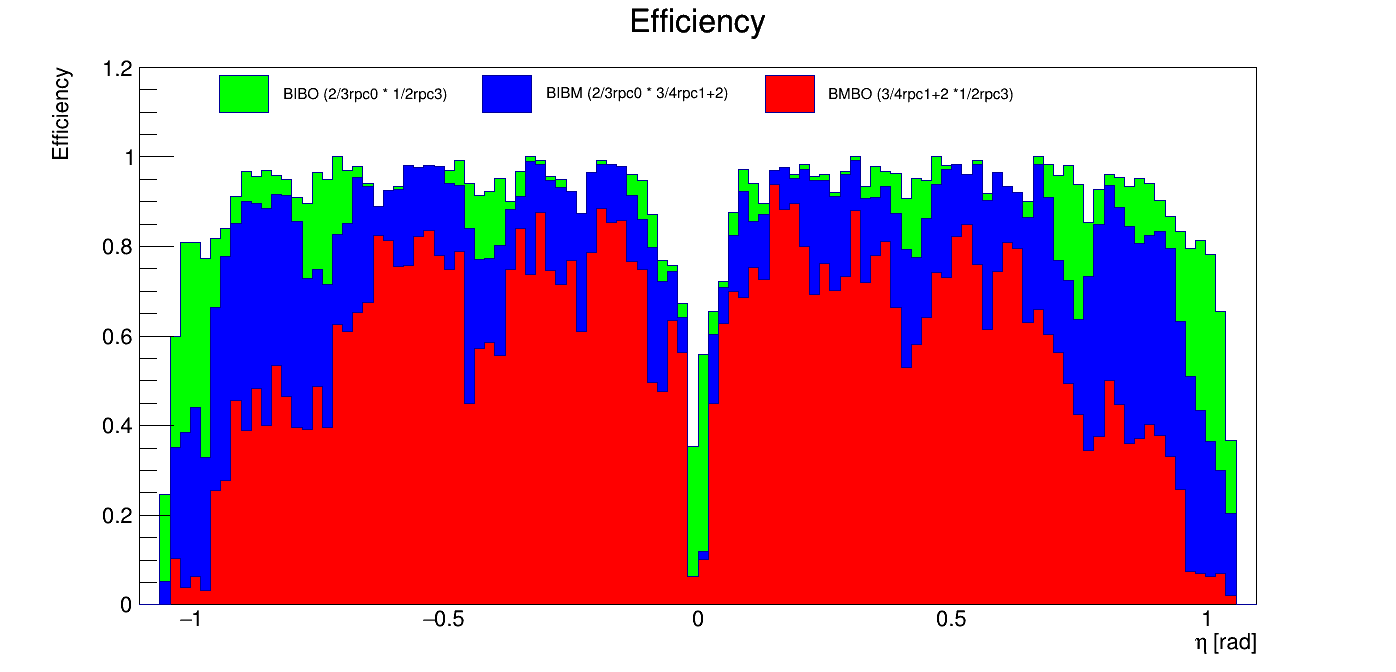
\includegraphics[width=1.1\textwidth]{Chapters/CH3/figures/h_eff}
	\caption{Efficiency times acceptance of the L0 barrel trigger for each trigger logic scheme, assuming the worst-case scenario with the hit digitization.}
	\label{fig:h_eff}
\end{figure}
\\Starting from the WCS scenario, other two studies have been performed on the L0 barrel trigger 
efficiency using simulations with RPC stations in various operational conditions: the first study is the  refurbish of BM and BO chambers (Section~\ref{sec:BMBO_retrofit}) and the second study is about the installation of BI chambers in the rail sectors 11 and 15 (Section~\ref{sec:BIRBIM_drop}).

\subsection{BM and BO retrofitting}
\label{sec:BMBO_retrofit}
In the Phase-II upgrade of the muon system, most of the readout electronics will
be replaced to make it faster and resistant to radiation.
An essential step is therefore to understand what would be the impact of the legacy BM/BO chambers with the new electronics.\\
In this first study, efficiencies of the "worst-case scenario" summarised in Table~\ref{tab:WCS}, are used, except for the following stations set to 100\% efficiency:
\renewcommand{\labelenumii}{\Lowercase{enumii}}
\begin{enumerate}
\item BML 7,
\item BOL 6,
\item BOS 6,
\item BOL 5.
\end{enumerate}
The products of muon trigger efficiency and acceptance for the BM and BO retrofitting are listed in Table~\ref{tab:allcasesBMBO}.\\
The trigger efficiency times acceptance is also presented in Figure~\ref{fig:allcasesBMBO} that compare the "worst-case scenario" with all the variants of the WCS, in which some stations are fixed to 100\% efficiency.\\
In the first analysed case, the most relevant effect on the trigger efficiency times acceptance is on the 3/4 chambers logic scheme, in particular for the Case 1b (BOL 6 100\%) the variation is +1.08\% compared to the "worst-case scenario".
\begin{table}[h]
	\begin{center}
		\small
		\begin{tabular}{l|c|c|c}
			\hline
			\multirow{2}{*}{\textbf{BM and BO efficiency (\%)}} & \multicolumn{3}{c}{\textbf{Trigger efficiency x acceptance (\%)}}\\
			\cline{2-4}   
			& \textbf{3/3 chambers} & \textbf{3/4 chambers} & \textbf{3/4 chambers + BIBO}\\
			\hline 
			WCS 												& 58.78 				& 83.27 		& 91.89\\
			Case 1a (BML 7 100\%) 								& +0.22                 & +0.26 		& +0.14\\
			Case 1b (BOL 6 100\%) 								& +0.13 				& +1.08 		& +0.53\\
			Case 1c (BOS 6 100\%) 								& +0.16 				& +0.51 		& +0.63\\
			Case 1d (BOL 5 100\%) 								& +0.23 				& +0.82 		& +0.41\\		
			\hline 
		\end{tabular} 
		\caption{Efficiency times acceptance for the L0 barrel trigger for different assumptions on the hit efficiency of the present RPC detectors. The “WCS” row corresponds to the scenario in which the efficiencies are listed in Table~\ref{tab:WCS}. The other rows correspond to the variants of the WCS, in which the efficiency of some stations are set to 100\%. The corresponding results of these variants, are expressed as variations to the WCS~\cite{Marcoccia:2693982}.} 
		\label{tab:allcasesBMBO}
	\end{center} 
\end{table} 

\begin{figure}[h]
	\centering
	\subfigure [3/3 chamber]{{\label{fig:allcasesBMBO_a}}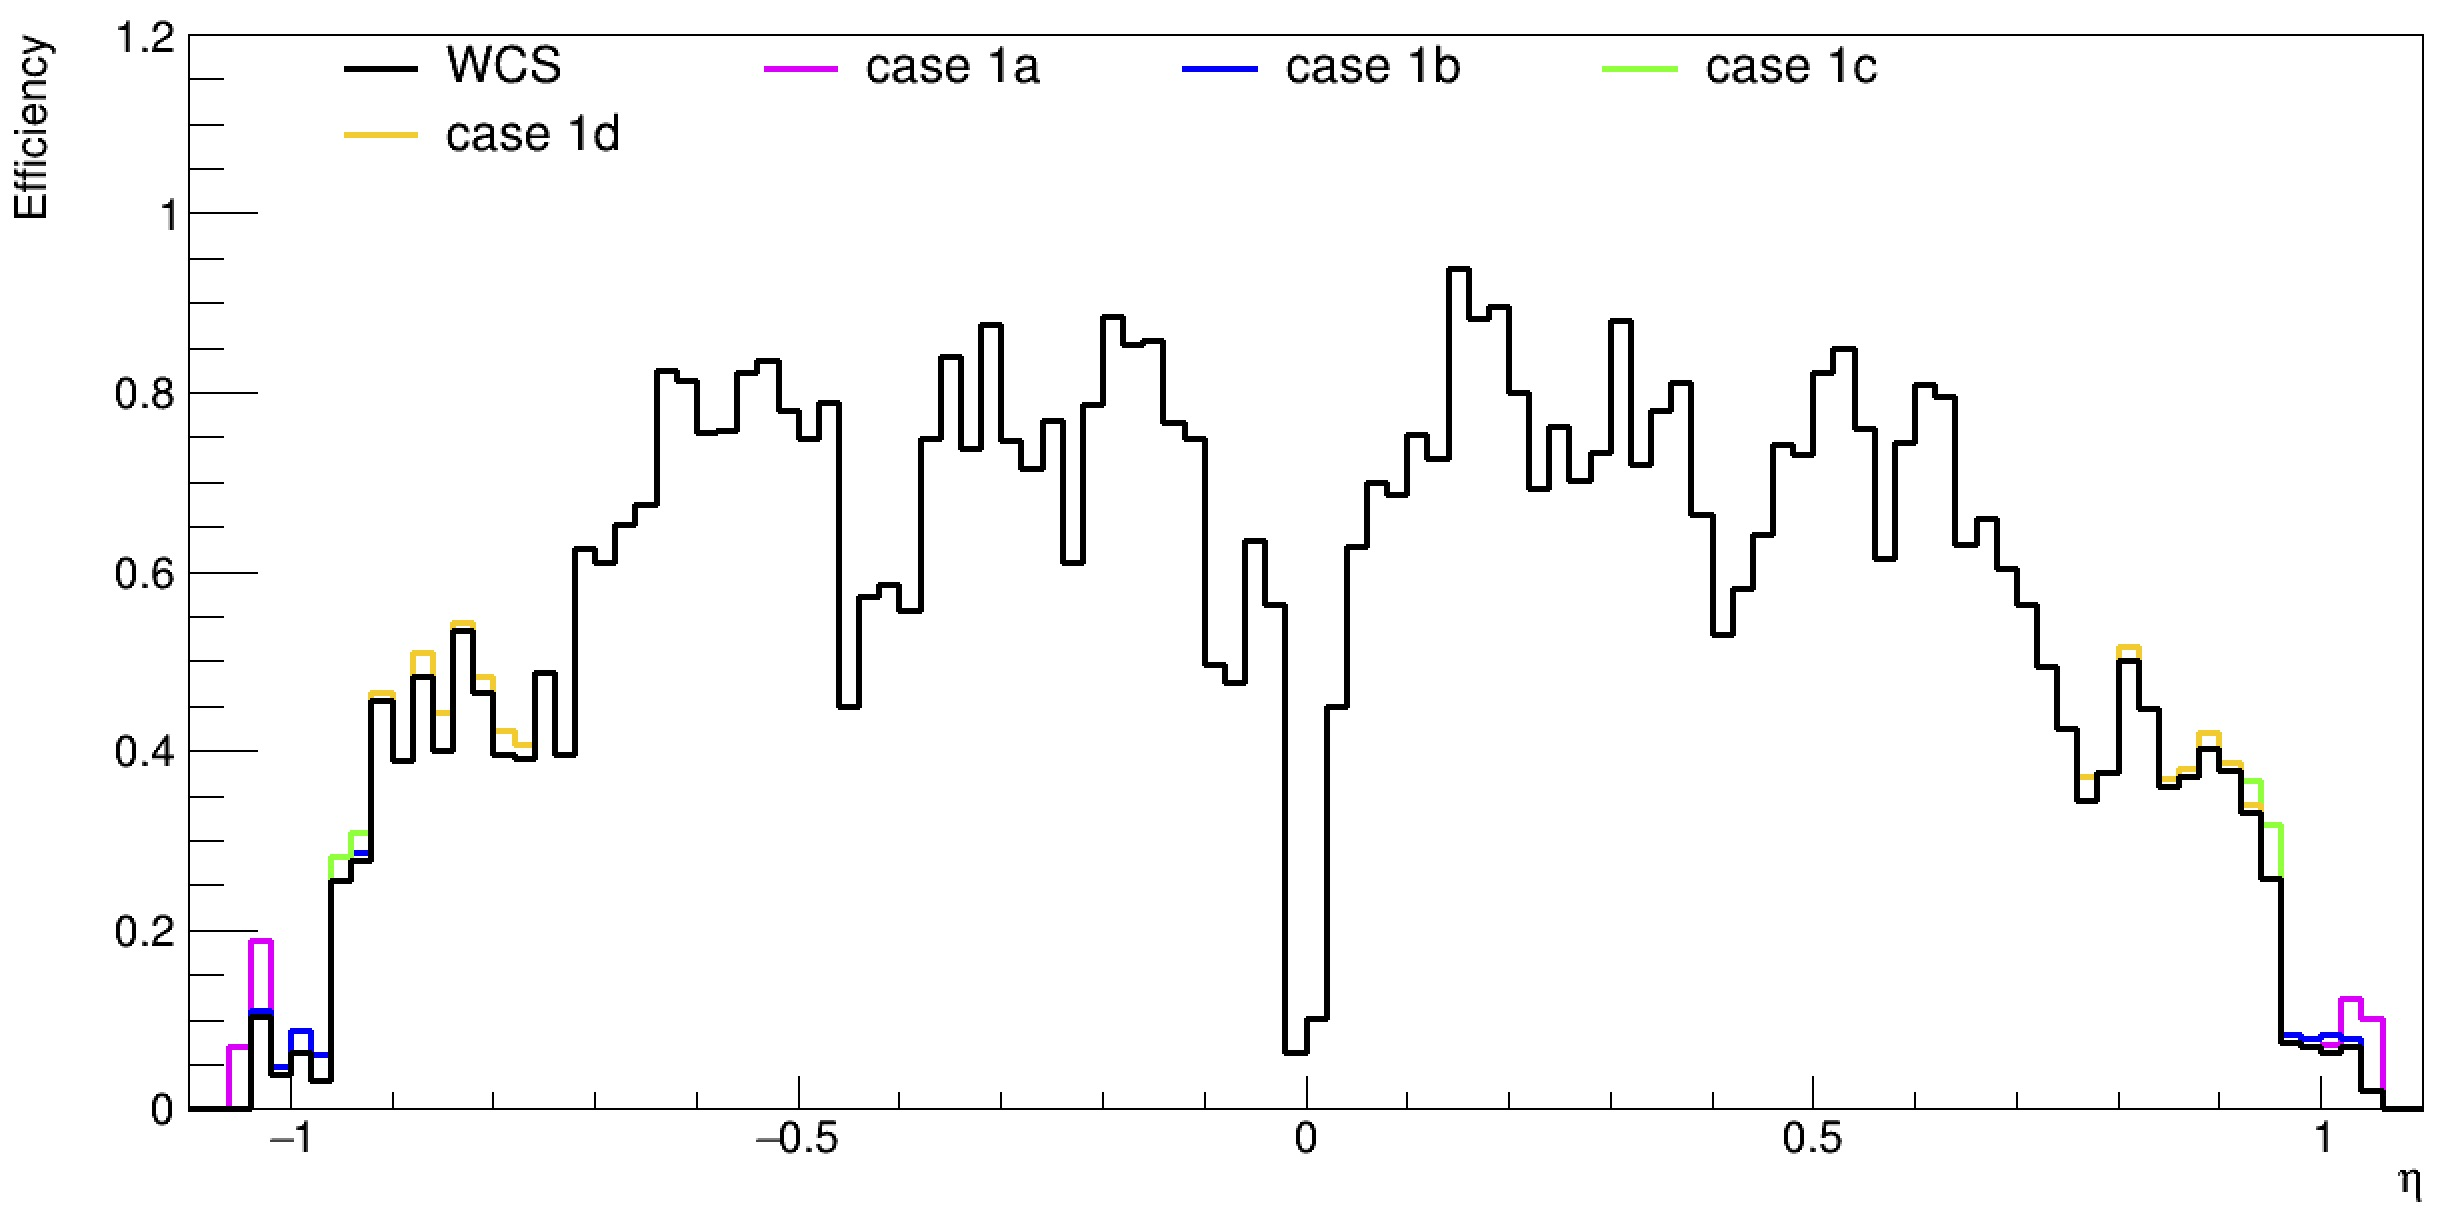
\includegraphics[width=0.95 \textwidth]{Chapters/CH3/figures/BMBO_firstCase}} 
\end{figure}	
\begin{figure}[h]
	\centering
	\subfigure [3/4 chambers]{{\label{fig:allcasesBMBO_b}}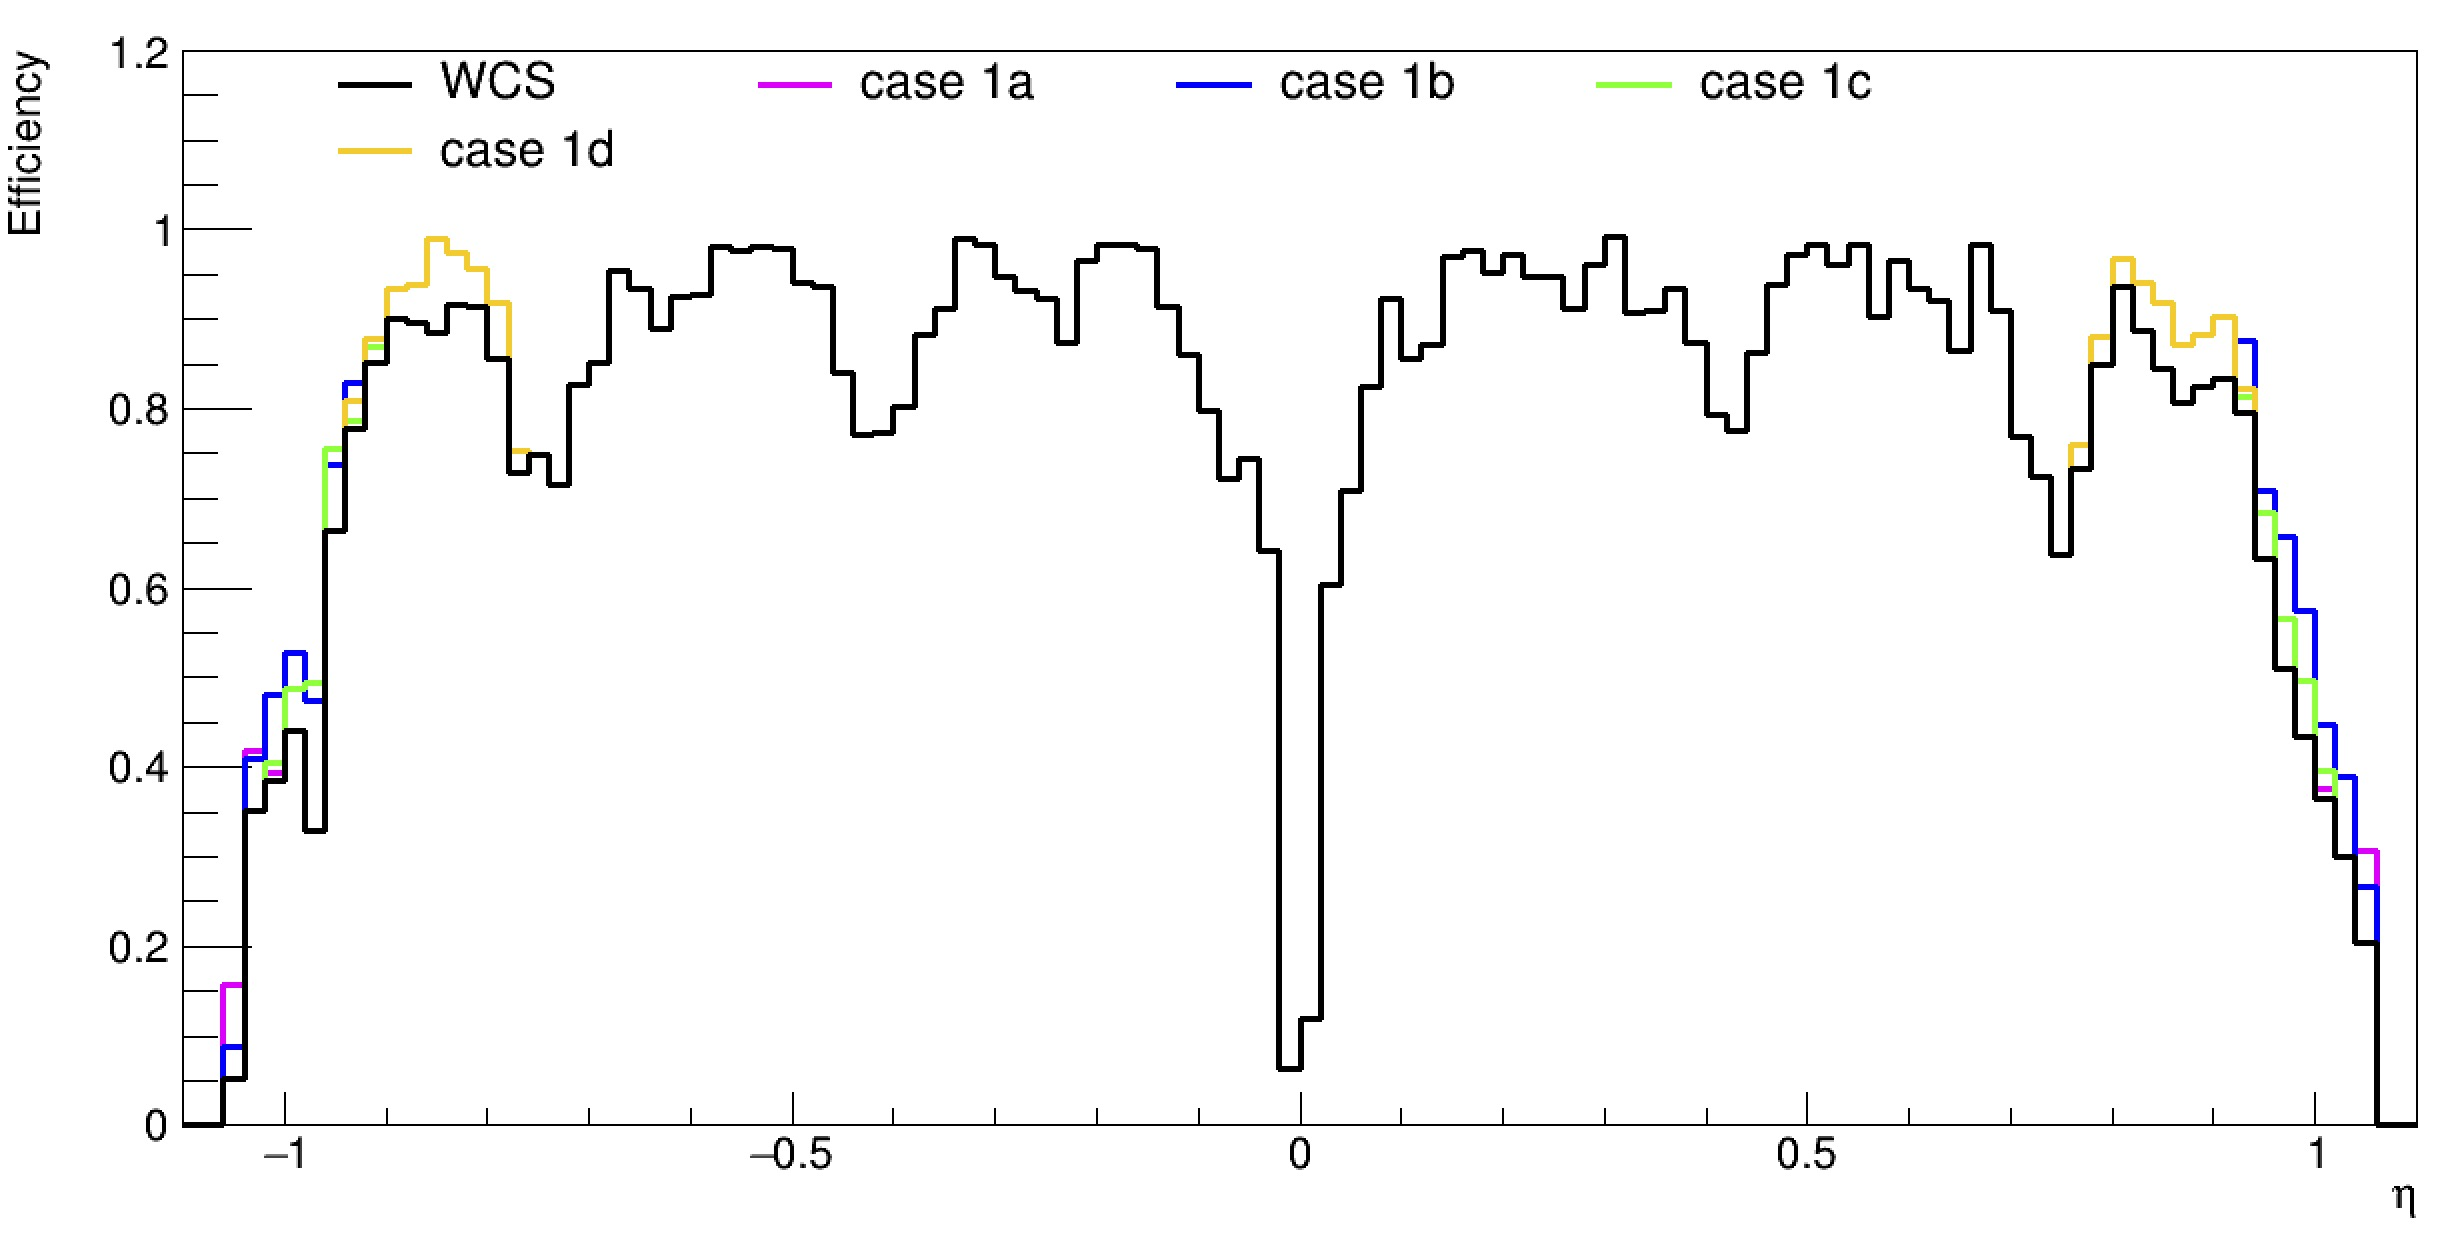
\includegraphics[width=0.95 \textwidth]{Chapters/CH3/figures/BIBM_firstCase}} 
	\subfigure [3/4 chambers + BIBO]{{\label{fig:allcasesBMBO_c}}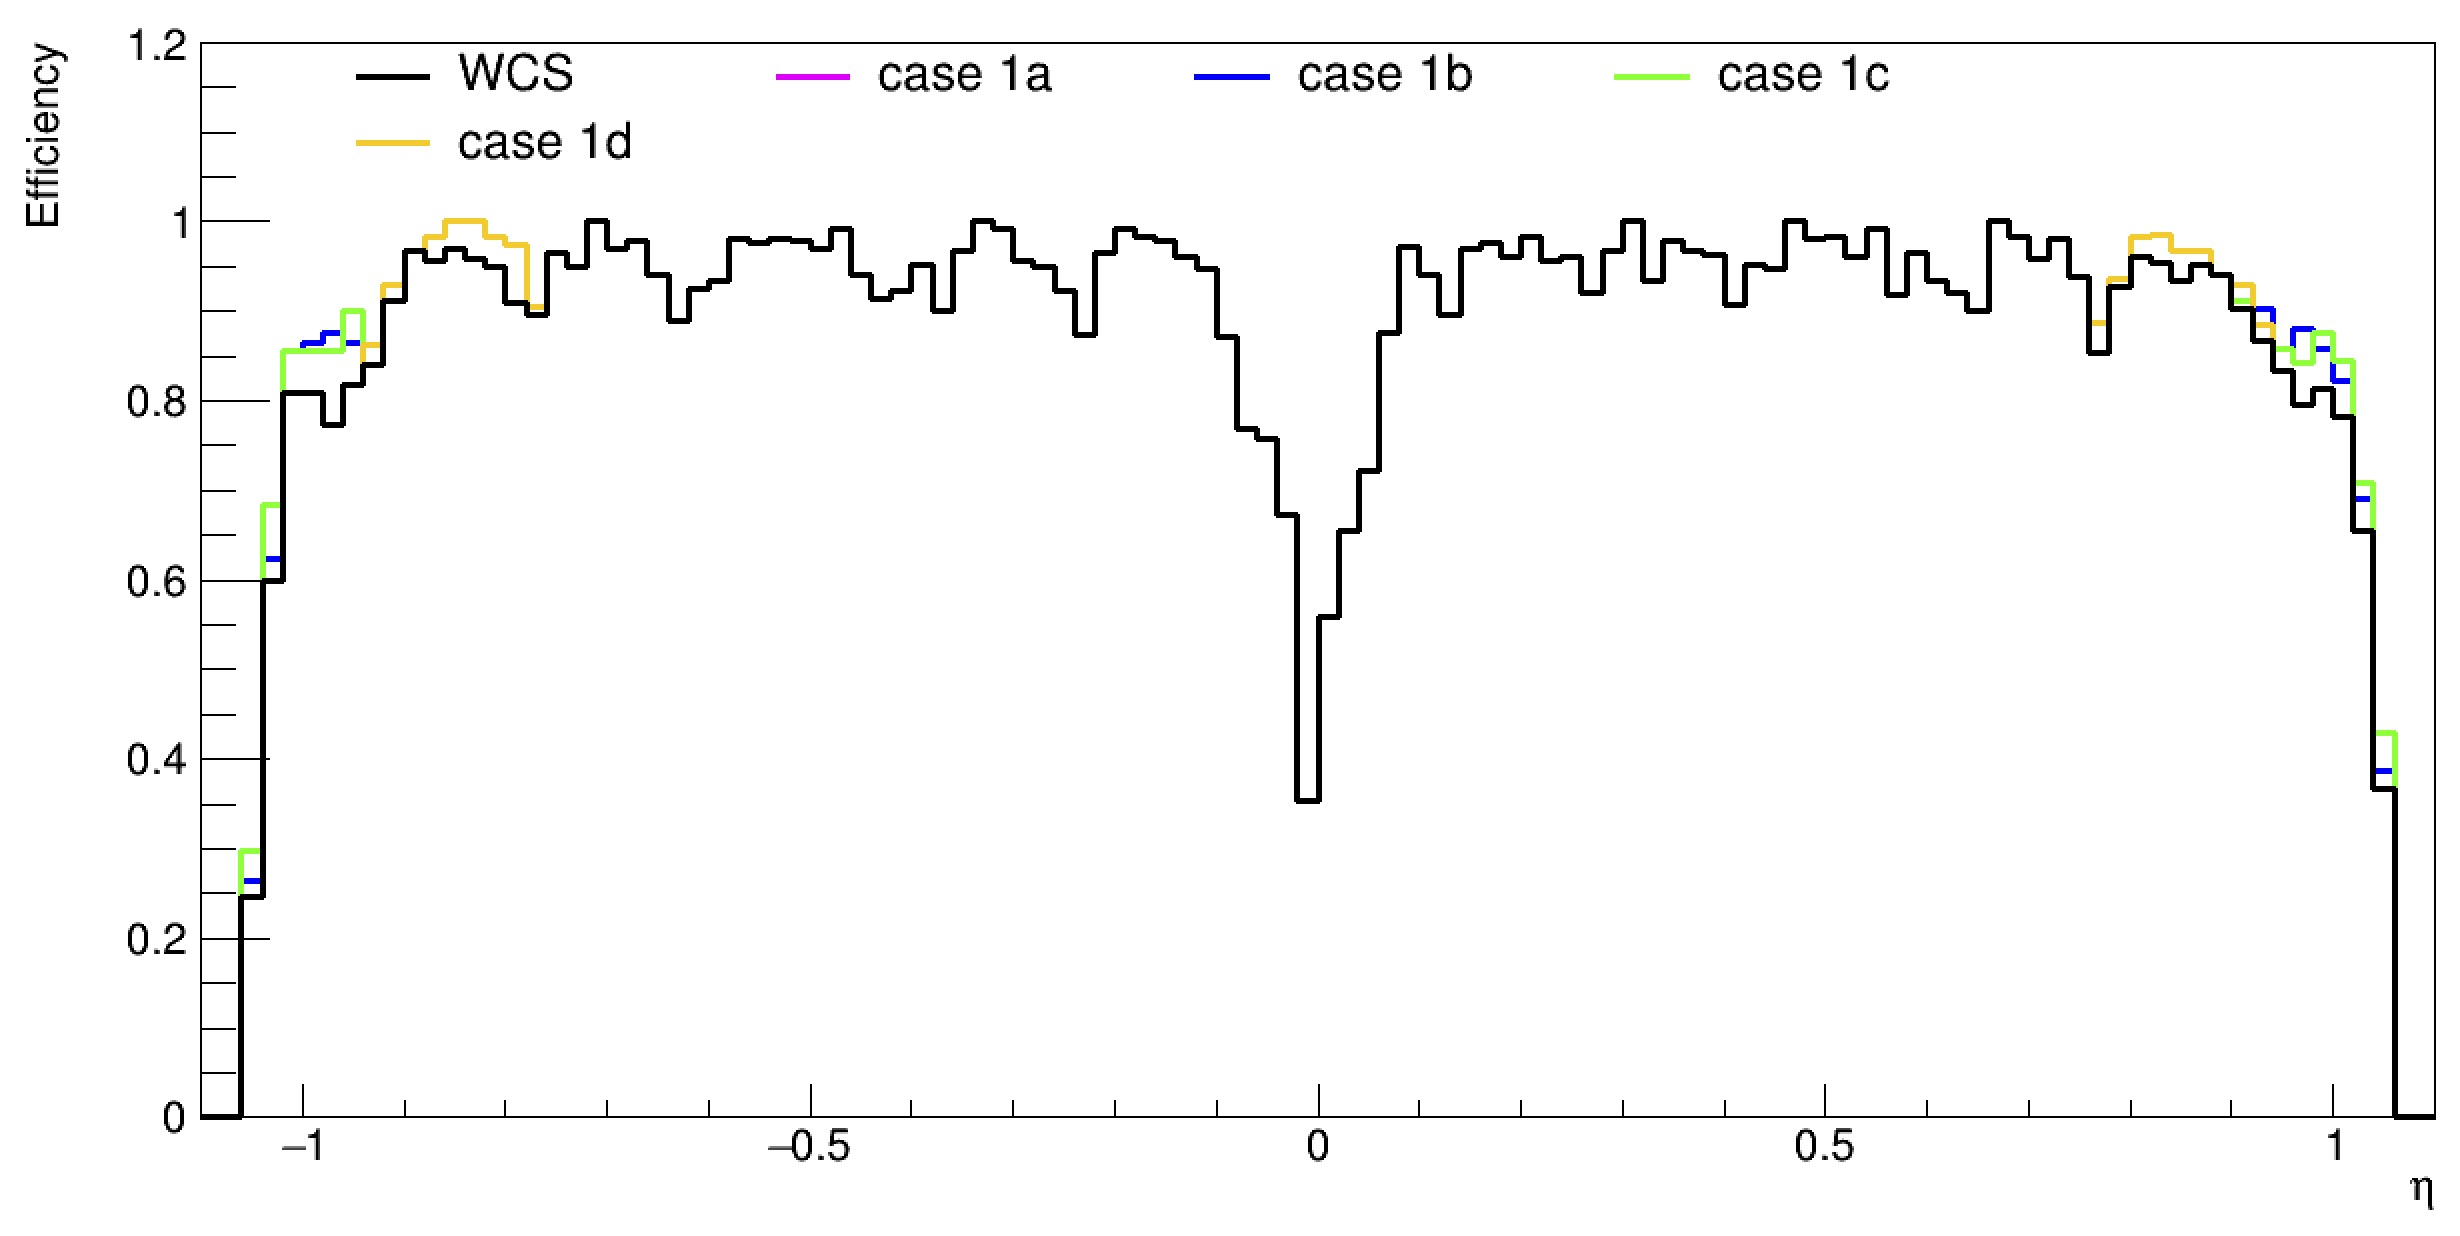
\includegraphics[width=0.95 \textwidth]{Chapters/CH3/figures/BIBO_firstCase}} 
	\caption{Efficiency times acceptance of the L0 barrel trigger compared to reconstructed muons with $p_{T} = 50$ GeV as a function of $\eta$ taking in to account all the variants of the WCS. The histograms show the efficiency of \subref{fig:allcasesBMBO_a} the existing 3/3 chambers trigger, of \subref{fig:allcasesBMBO_b}  the 3/4 chambers trigger including the BI layer, and \subref{fig:allcasesBMBO_c}  the additional gain from the BI-BO trigger. Efficiency times acceptance is defined as the fraction of reconstructed muons accepted by the trigger, using a simulation that includes the RPC detector efficiency~\cite{Marcoccia:2693982}.}
	\label{fig:allcasesBMBO}
\end{figure}

\FloatBarrier
\subsection{Dropping BIR and BIM chambers}
\label{sec:BIRBIM_drop}
Since the installation of the RPCs in the sectors 11 and 15  seems to be very hard, another special case was performed simulating a scenario in which BIM and BIR RPC are not installed in these sectors.\\
The products of muon trigger efficiency and acceptance for this second study are listed in Table~\ref{tab:allcasesBIRBIM}.\\
The results are also presented in Figure~\ref{fig:allcasesBIRBIM} that compares the "worst-case scenario" with this second case, in which BIM and BIR are turned off.
The efficiency distributions show that the absence of BIR and BIM has the most relevant effect on the 3/4 chambers + BIBO logic scheme with a corresponding variation of -3.11\%.

\begin{table}[h]
	\begin{center}
		\small
		\begin{tabular}{l|c|c|c}
			\hline
			\multirow{2}{*}{\textbf{BM and BO efficiency (\%)}} & \multicolumn{3}{c}{\textbf{Trigger efficiency x acceptance (\%)}}\\
			\cline{2-4}   
			& \textbf{3/3 chambers} & \textbf{3/4 chambers} & \textbf{3/4 chambers + BIBO}\\
			\hline 
			WCS 												& 58.78 				& 83.27 				& 91.89\\
			Case 2  (BIM BIR off)								& +0.03 			   	& -2.70 				& -3.11\\
			\hline 
		\end{tabular} 
		\caption{Efficiency times acceptance for the L0 barrel trigger for different assumptions on the hit efficiency of the present RPC detectors. The WCS row corresponds to the scenario in which the efficiencies are listed in Table~\ref{tab:WCS}. The row "Case 2" corresponds to the case in which the RPCs in the sectors 11-15 (BIM and BIR) are turned off. The corresponding results of the Case 2, are expressed as variations to the WCS~\cite{Marcoccia:2693982}.} 
		\label{tab:allcasesBIRBIM}
	\end{center} 
\end{table} 
%\subfloat [Case 1a: BML 7 100\%] {\includegraphics[width=.5 \textwidth]{figures/h_eff_1a}} 
%\subfloat [Case 1b: BOL 6 100\%] {\includegraphics[width=.5 \textwidth]{figures/h_eff_1b}} \\
%\subfloat [Case 1c: BOS 6 100\%] {\includegraphics[width=.5 \textwidth]{figures/h_eff_1c}} 
%\subfloat [Case 1d: BOL 5 100\%] {\includegraphics[width=.5 \textwidth]{figures/h_eff_1d}} \\
%\subfloat [Case  2: BIM BIR off]    {\includegraphics[width=.5 \textwidth]{figures/h_eff_2}}  

\begin{figure}[h]
	\centering
	\subfigure [3/3 chambers]{\label{fig:allcasesBIRBIM_a}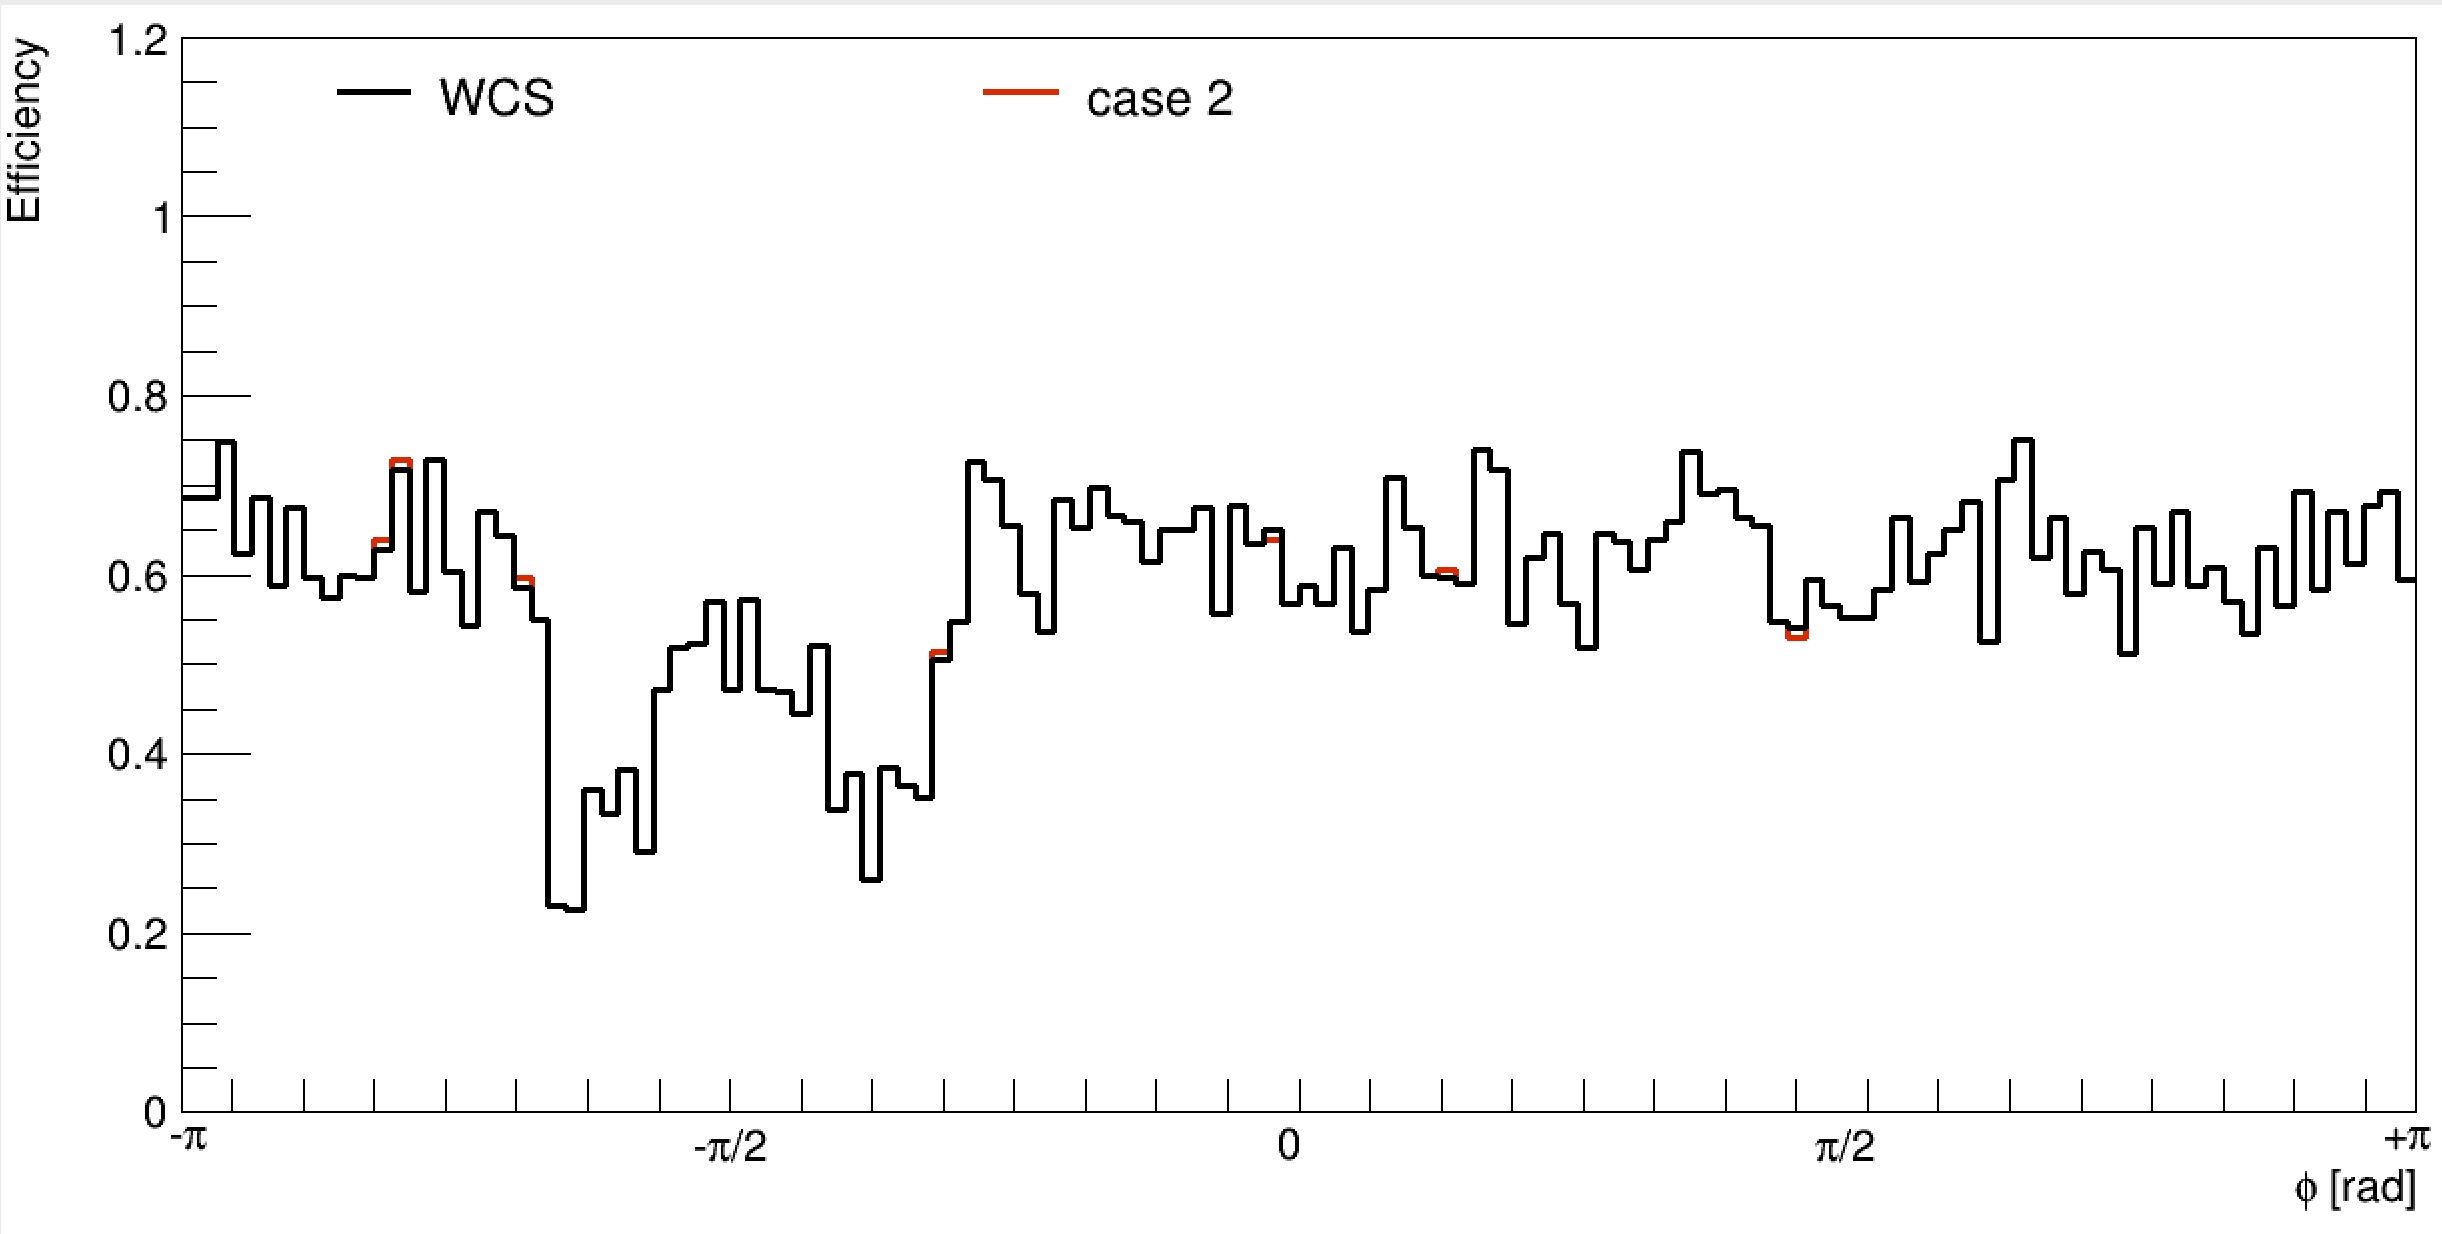
\includegraphics[width=0.95 \textwidth]{Chapters/CH3/figures/BMBO_secondCase_phi}} 
\end{figure}	

\begin{figure}[h]
	\centering	
	\subfigure [3/4 chambers]{\label{fig:allcasesBIRBIM_b}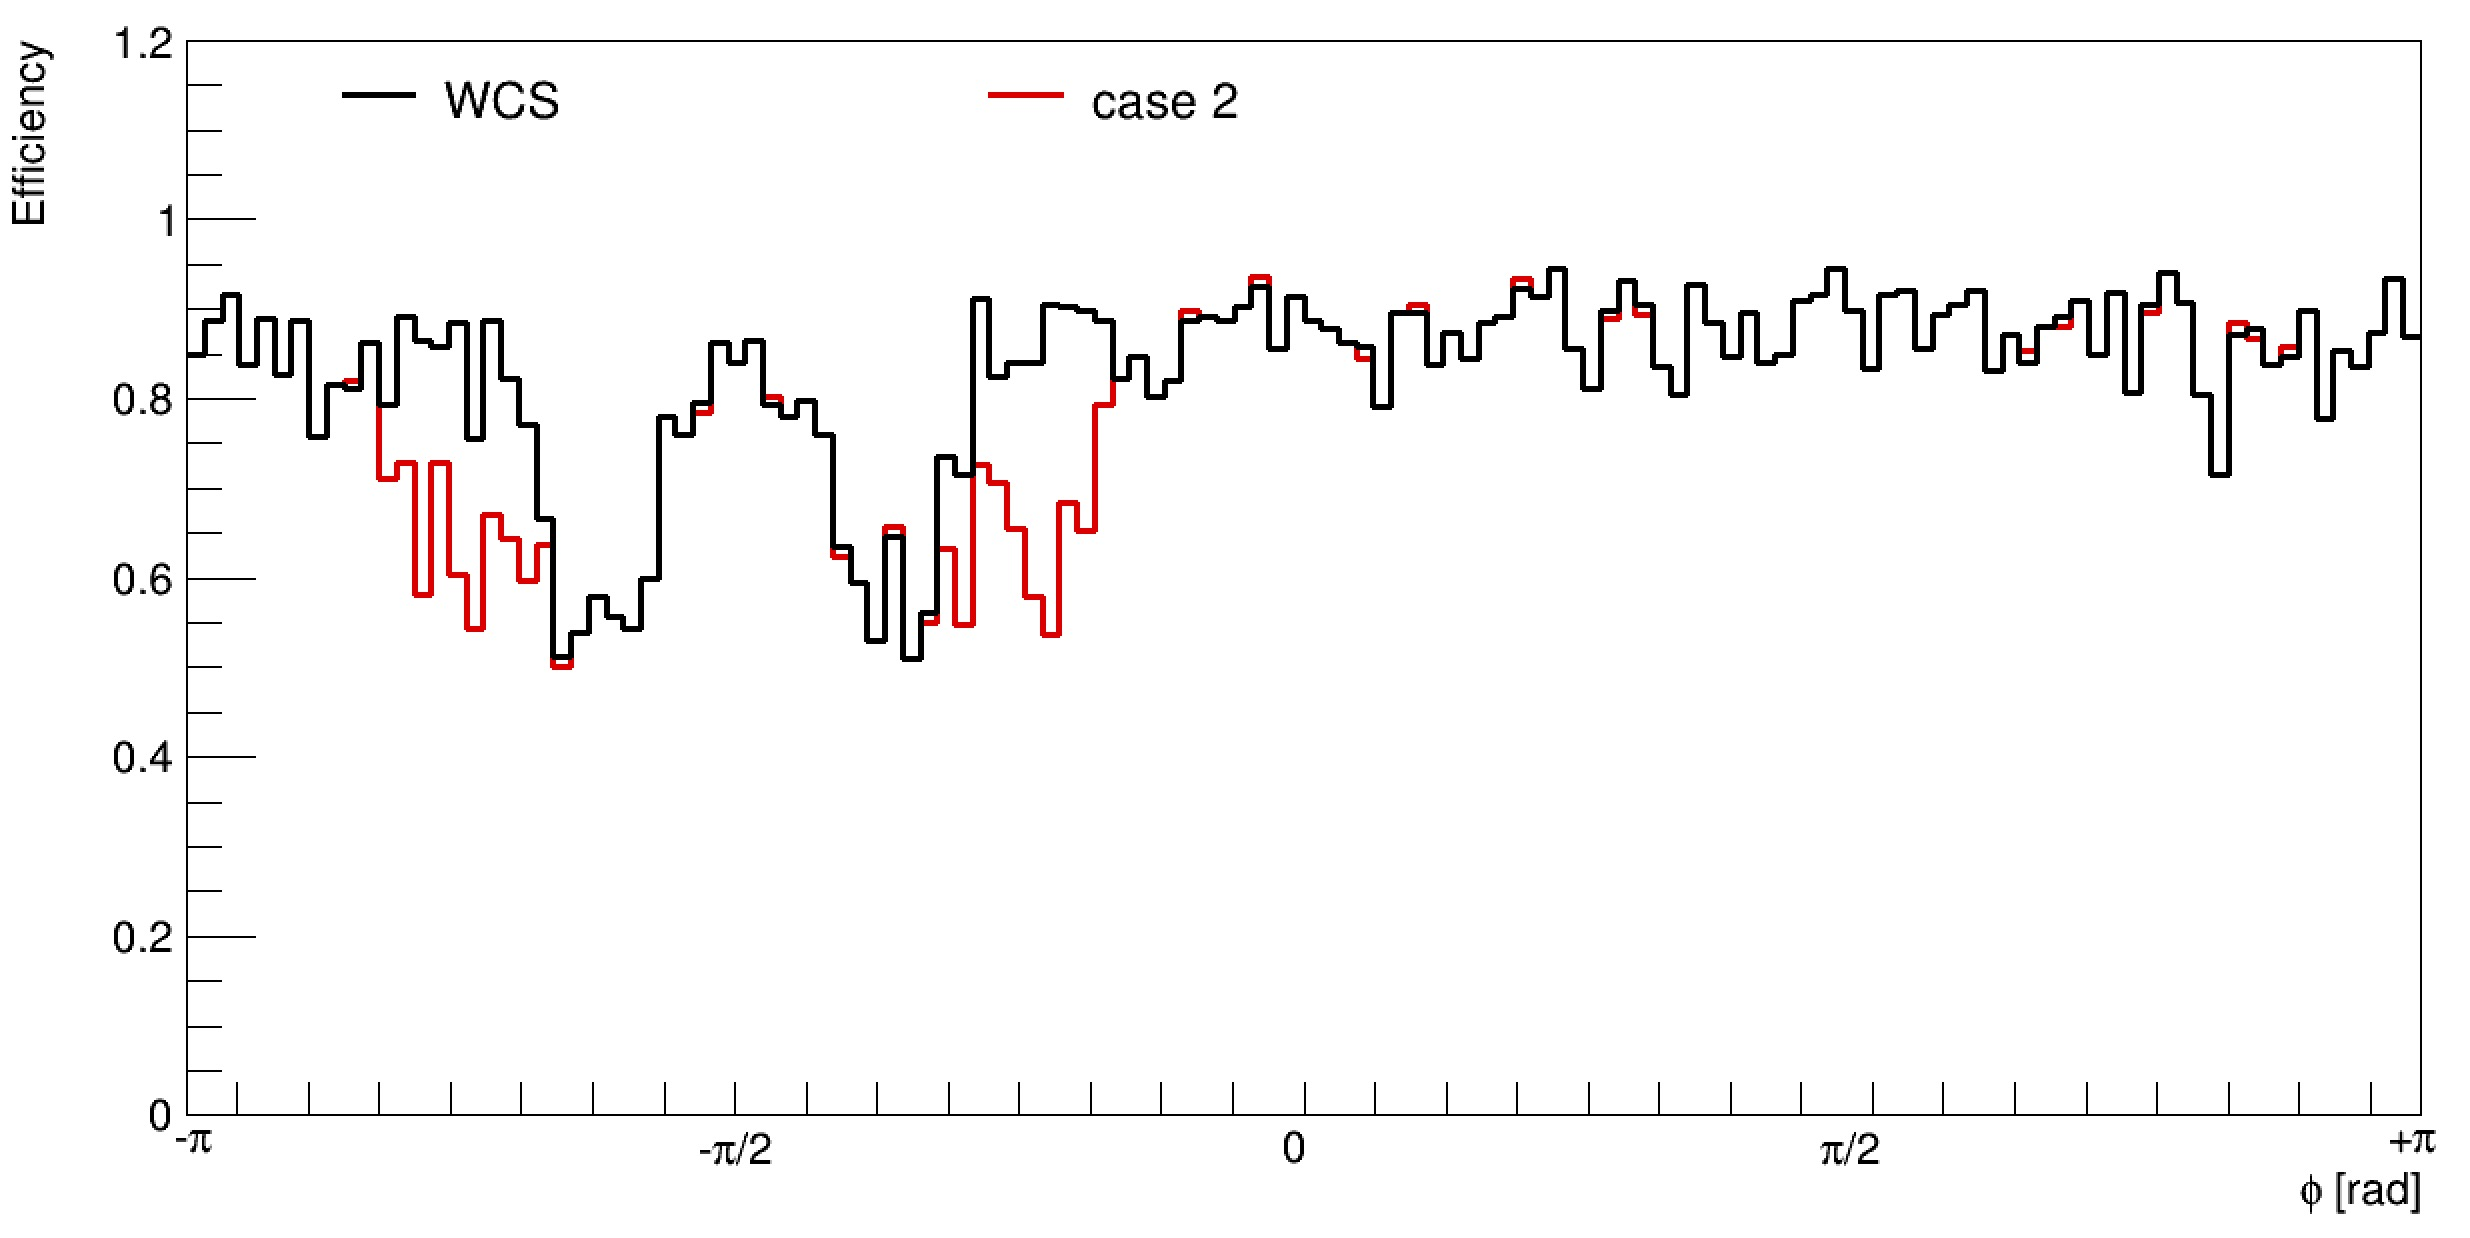
\includegraphics[width=0.95 \textwidth]{Chapters/CH3/figures/BIBM_secondCase_phi}} 
	\subfigure [3/4 chambers + BIBO]{\label{fig:allcasesBIRBIM_c}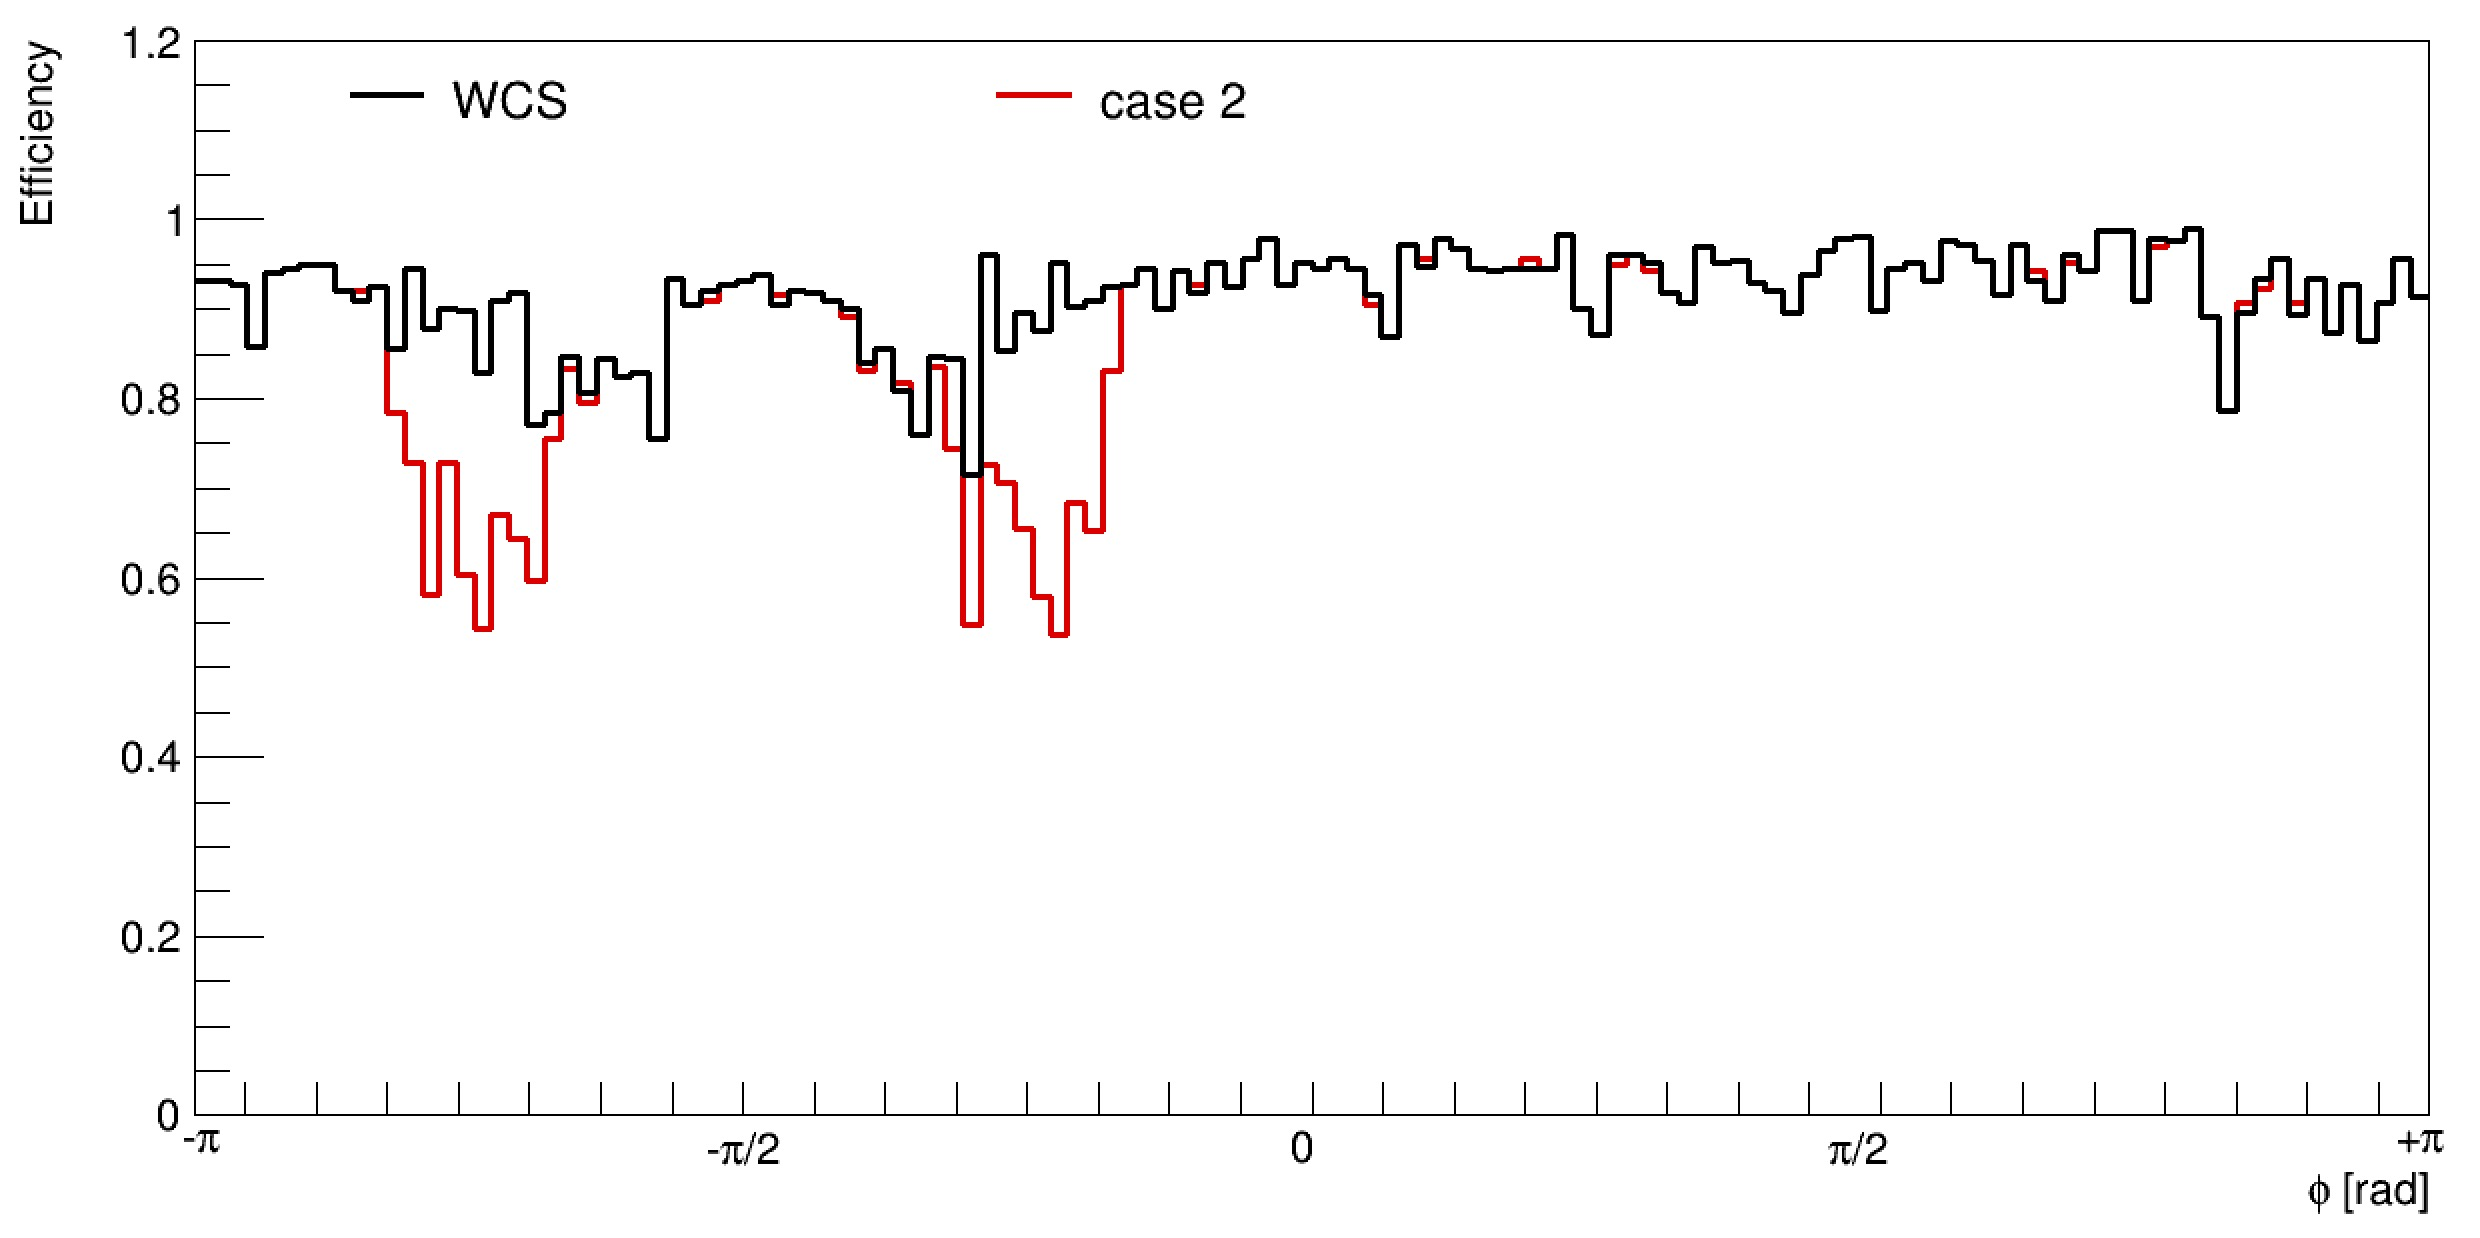
\includegraphics[width=0.95 \textwidth]{Chapters/CH3/figures/BIBO_secondCase_phi}} 
	\caption{Efficiency times acceptance of the L0 barrel trigger compared to reconstructed muons with $p_{T} = 50$ GeV as a function of $\phi$. The histograms show the efficiency of \subref{fig:allcasesBIRBIM_a}  the existing 3/3 chambers trigger, of \subref{fig:allcasesBIRBIM_b} the 3/4 chambers trigger including the BI layer, and \subref{fig:allcasesBIRBIM_c} the additional gain from the BI-BO trigger. Efficiency times acceptance is defined as the fraction of reconstructed muons accepted by the trigger, using a simulation that includes the RPC detector efficiency~\cite{Marcoccia:2693982}.}
	\label{fig:allcasesBIRBIM}
\end{figure}	
\FloatBarrier

\section{Summary and considerations }
\label{sec:concl_QT}
The works described in this chapter aimed at a new simulation of the RPC in the BI region.
They involved the construction of a model:
\begin{itemize}
\item for the definition of the cluster size, which is important for creating a simulation as realistic as possible;
\item to define a variable that represents the time taken by the particle to pass through the detector, which is important because it is one of the discriminating variables in the algorithm's selection of hits.
\end{itemize}
The new developed model results in agreement with the required technical characteristics of the RPCs for Phase-II, described in the Technical Design Report~\cite {TDR}.\\
A more realistic simulation of the RPCs is now available for further studies.
\vspace{\baselineskip}
\\Using this model, L0 barrel trigger efficiency studies were performed in the following two scenarios:
\begin{enumerate}
\item the refurbish of BM and BO chambers, to understand what would be the impact of the legacy BM / BO chambers with the new electronics;
\item the drop of BIR and BIM chambers, given that the installation of the RPCs in the sectors 11 and 15 seems to be very hard.
\end{enumerate}
The first scenario gives an estimation of the improvements by replacing the electronics. Moreover, the most significant expected improvement is from BOL6.\\
The second scenario showed that there is a significant loss of efficiency if the collaboration decides to don't install the RPC in sectors 11 and 15.\\
These two studies will help plan the work for the Phase-II upgrade. 